% Options for packages loaded elsewhere
\PassOptionsToPackage{unicode}{hyperref}
\PassOptionsToPackage{hyphens}{url}
%
\documentclass[
  man,floatsintext]{apa6}
\usepackage{amsmath,amssymb}
\usepackage{lmodern}
\usepackage{iftex}
\ifPDFTeX
  \usepackage[T1]{fontenc}
  \usepackage[utf8]{inputenc}
  \usepackage{textcomp} % provide euro and other symbols
\else % if luatex or xetex
  \usepackage{unicode-math}
  \defaultfontfeatures{Scale=MatchLowercase}
  \defaultfontfeatures[\rmfamily]{Ligatures=TeX,Scale=1}
\fi
% Use upquote if available, for straight quotes in verbatim environments
\IfFileExists{upquote.sty}{\usepackage{upquote}}{}
\IfFileExists{microtype.sty}{% use microtype if available
  \usepackage[]{microtype}
  \UseMicrotypeSet[protrusion]{basicmath} % disable protrusion for tt fonts
}{}
\makeatletter
\@ifundefined{KOMAClassName}{% if non-KOMA class
  \IfFileExists{parskip.sty}{%
    \usepackage{parskip}
  }{% else
    \setlength{\parindent}{0pt}
    \setlength{\parskip}{6pt plus 2pt minus 1pt}}
}{% if KOMA class
  \KOMAoptions{parskip=half}}
\makeatother
\usepackage{xcolor}
\usepackage{graphicx}
\makeatletter
\def\maxwidth{\ifdim\Gin@nat@width>\linewidth\linewidth\else\Gin@nat@width\fi}
\def\maxheight{\ifdim\Gin@nat@height>\textheight\textheight\else\Gin@nat@height\fi}
\makeatother
% Scale images if necessary, so that they will not overflow the page
% margins by default, and it is still possible to overwrite the defaults
% using explicit options in \includegraphics[width, height, ...]{}
\setkeys{Gin}{width=\maxwidth,height=\maxheight,keepaspectratio}
% Set default figure placement to htbp
\makeatletter
\def\fps@figure{htbp}
\makeatother
\setlength{\emergencystretch}{3em} % prevent overfull lines
\providecommand{\tightlist}{%
  \setlength{\itemsep}{0pt}\setlength{\parskip}{0pt}}
\setcounter{secnumdepth}{-\maxdimen} % remove section numbering
% Make \paragraph and \subparagraph free-standing
\ifx\paragraph\undefined\else
  \let\oldparagraph\paragraph
  \renewcommand{\paragraph}[1]{\oldparagraph{#1}\mbox{}}
\fi
\ifx\subparagraph\undefined\else
  \let\oldsubparagraph\subparagraph
  \renewcommand{\subparagraph}[1]{\oldsubparagraph{#1}\mbox{}}
\fi
\newlength{\cslhangindent}
\setlength{\cslhangindent}{1.5em}
\newlength{\csllabelwidth}
\setlength{\csllabelwidth}{3em}
\newlength{\cslentryspacingunit} % times entry-spacing
\setlength{\cslentryspacingunit}{\parskip}
\newenvironment{CSLReferences}[2] % #1 hanging-ident, #2 entry spacing
 {% don't indent paragraphs
  \setlength{\parindent}{0pt}
  % turn on hanging indent if param 1 is 1
  \ifodd #1
  \let\oldpar\par
  \def\par{\hangindent=\cslhangindent\oldpar}
  \fi
  % set entry spacing
  \setlength{\parskip}{#2\cslentryspacingunit}
 }%
 {}
\usepackage{calc}
\newcommand{\CSLBlock}[1]{#1\hfill\break}
\newcommand{\CSLLeftMargin}[1]{\parbox[t]{\csllabelwidth}{#1}}
\newcommand{\CSLRightInline}[1]{\parbox[t]{\linewidth - \csllabelwidth}{#1}\break}
\newcommand{\CSLIndent}[1]{\hspace{\cslhangindent}#1}
\ifLuaTeX
\usepackage[bidi=basic]{babel}
\else
\usepackage[bidi=default]{babel}
\fi
\babelprovide[main,import]{english}
% get rid of language-specific shorthands (see #6817):
\let\LanguageShortHands\languageshorthands
\def\languageshorthands#1{}
% Manuscript styling
\usepackage{upgreek}
\captionsetup{font=singlespacing,justification=justified}

% Table formatting
\usepackage{longtable}
\usepackage{lscape}
% \usepackage[counterclockwise]{rotating}   % Landscape page setup for large tables
\usepackage{multirow}		% Table styling
\usepackage{tabularx}		% Control Column width
\usepackage[flushleft]{threeparttable}	% Allows for three part tables with a specified notes section
\usepackage{threeparttablex}            % Lets threeparttable work with longtable

% Create new environments so endfloat can handle them
% \newenvironment{ltable}
%   {\begin{landscape}\centering\begin{threeparttable}}
%   {\end{threeparttable}\end{landscape}}
\newenvironment{lltable}{\begin{landscape}\centering\begin{ThreePartTable}}{\end{ThreePartTable}\end{landscape}}

% Enables adjusting longtable caption width to table width
% Solution found at http://golatex.de/longtable-mit-caption-so-breit-wie-die-tabelle-t15767.html
\makeatletter
\newcommand\LastLTentrywidth{1em}
\newlength\longtablewidth
\setlength{\longtablewidth}{1in}
\newcommand{\getlongtablewidth}{\begingroup \ifcsname LT@\roman{LT@tables}\endcsname \global\longtablewidth=0pt \renewcommand{\LT@entry}[2]{\global\advance\longtablewidth by ##2\relax\gdef\LastLTentrywidth{##2}}\@nameuse{LT@\roman{LT@tables}} \fi \endgroup}

% \setlength{\parindent}{0.5in}
% \setlength{\parskip}{0pt plus 0pt minus 0pt}

% Overwrite redefinition of paragraph and subparagraph by the default LaTeX template
% See https://github.com/crsh/papaja/issues/292
\makeatletter
\renewcommand{\paragraph}{\@startsection{paragraph}{4}{\parindent}%
  {0\baselineskip \@plus 0.2ex \@minus 0.2ex}%
  {-1em}%
  {\normalfont\normalsize\bfseries\itshape\typesectitle}}

\renewcommand{\subparagraph}[1]{\@startsection{subparagraph}{5}{1em}%
  {0\baselineskip \@plus 0.2ex \@minus 0.2ex}%
  {-\z@\relax}%
  {\normalfont\normalsize\itshape\hspace{\parindent}{#1}\textit{\addperi}}{\relax}}
\makeatother

% \usepackage{etoolbox}
\makeatletter
\patchcmd{\HyOrg@maketitle}
  {\section{\normalfont\normalsize\abstractname}}
  {\section*{\normalfont\normalsize\abstractname}}
  {}{\typeout{Failed to patch abstract.}}
\patchcmd{\HyOrg@maketitle}
  {\section{\protect\normalfont{\@title}}}
  {\section*{\protect\normalfont{\@title}}}
  {}{\typeout{Failed to patch title.}}
\makeatother

\usepackage{xpatch}
\makeatletter
\xapptocmd\appendix
  {\xapptocmd\section
    {\addcontentsline{toc}{section}{\appendixname\ifoneappendix\else~\theappendix\fi\\: #1}}
    {}{\InnerPatchFailed}%
  }
{}{\PatchFailed}
\keywords{demand characteristics, hypothesis awareness, placebo effect, research methods, meta-analysis}
\usepackage{csquotes}
\ifLuaTeX
  \usepackage{selnolig}  % disable illegal ligatures
\fi
\IfFileExists{bookmark.sty}{\usepackage{bookmark}}{\usepackage{hyperref}}
\IfFileExists{xurl.sty}{\usepackage{xurl}}{} % add URL line breaks if available
\urlstyle{same} % disable monospaced font for URLs
\hypersetup{
  pdftitle={A quantitative review of demand characteristics and their underlying mechanisms},
  pdfauthor={Nicholas A. Coles1 \& Michael C. Frank2},
  pdflang={en-EN},
  pdfkeywords={demand characteristics, hypothesis awareness, placebo effect, research methods, meta-analysis},
  hidelinks,
  pdfcreator={LaTeX via pandoc}}

\title{A quantitative review of demand characteristics and their underlying mechanisms}
\author{Nicholas A. Coles\textsuperscript{1} \& Michael C. Frank\textsuperscript{2}}
\date{}


\shorttitle{Demand characteristics meta-analysis}

\authornote{

All materials, data, and code are available at \url{http://github.com/ColesNicholas/metaware}. We thank Morgan H. Wyatt for his assistance on the project. This work was supported by the John Templeton Foundation (grant \# 62295). The funder had no role in the preparation of the manuscript or decision to publish.

Correspondence concerning this article should be addressed to Nicholas A. Coles, Cordura Hall, 210 Panama St, Stanford, CA 94305. E-mail: \href{mailto:ncoles@stanford.edu}{\nolinkurl{ncoles@stanford.edu}}

}

\affiliation{\vspace{0.5cm}\textsuperscript{1} Center for the Study of Language and Information, Stanford University\\\textsuperscript{2} Department of Psychology, Stanford University}

\abstract{%
Demand characteristics are a fundamental methodological concern in experimental psychology. Yet, little is known about the direction, magnitude, consistency, and mechanisms underlying their effects. We conducted a meta-analysis of 195 effect sizes from 40 studies that provided strict experimental tests of demand effects by manipulating the hypothesis communicated to participants. Demand characteristics tended to produce small increases in hypothesis-consistent responding (\emph{d} = 0.22, 95\% CI {[}0.11, 0.33{]}). However, these effects were extremely heterogeneous (between-study \(\tau\) = 0.30; within-study \(\sigma\) = 0.20), with the estimated distribution of true effects ranging from \emph{d} = 1.91 (a large increase in hypothesis-consistent responding) to \emph{d} = -1.67 (a large increase in hypothesis-\emph{in}consistent responding). Contra prior predictions, we did not find evidence that demand effects were driven participants' motivation and opportunity to adjust their responses. We did, however, find robust evidence that such effects are driven by participants' beliefs, as in placebo effects. Similar findings emerged in a direct replication of a study included in the meta-analysis. Taken together, results challenge conventional distinctions between demand characteristics and placebo effects. Furthermore, they underscore the importance of controlling for both response bias and placebo effects in experimental work.
}



\begin{document}
\maketitle

Imagine that a mysterious person approaches you and begins telling you about a new method for understanding humans. They explain that this method is useful for estimating causal relationships, but add that it can sometimes be thrown off by a methodological artifact. They explain that this artifact sometimes causes researchers to detect an effect that's not real, and other times causes them to miss an effect that is real. They add it that it sometimes biases relationships upward and other times downward. They then offer a confession: the artifact doesn't always appear, but they don't understand how it works. Sometimes the artifact seems to matter, other times it doesn't -- and its underlying mechanisms are poorly understood. If this scenario were real, it seems like this concern would call the whole method into question. However, perhaps experimental psychologists should not be so quick to judge because we too deal with a difficult-to-understand methodological artifact: \emph{demand characteristics}.

In a seminal paper, Martin Orne (1962) argued that human subjects are \emph{not} passive responders to the experimental context (a common assumption in the early history of experimental psychology). Instead, he suggested that participants are perceptive to demand characteristics -- ``cues which convey an experimental hypothesis'' -- and are motivated to use these cues to help the experimenter confirm their hypothesis (Orne, 1962, p. 779). This idea was controversial at first, with some researchers suggesting that the concern was vague and/or overblown (e.g., Berkowitz, 1971; Kruglanski, 1975; Milgram, 1972). Nonetheless, over the next 60 years, demand characteristics have become a literal textbook methodological concern in experimental psychology (Sharpe \& Whelton, 2016).

Orne initially focused on evidence that demand characteristics can lead to false positives -- such as patients exhibiting sham symptoms of hypnosis (Orne, 1959). But demand characteristics can also lead to false negatives. For example, participants will ignore visual cues of depth when they believe that doing so is the purpose of the experiment (Hayes \& King, 1967). In addition to creating inferential errors, demand characteristics can bias estimates of causal relationships. For example, the effect of facial poses on self-reported emotion can be amplified \emph{or} attenuated depending on whether the experimenter communicates expectations of positive or nil effects (Coles, Gaertner, Frohlich, Larsen, \& Basnight-Brown, 2022). However, demand characteristics do not always matter. For example, manipulations of the communicated hypothesis have consistently failed to impact participants' responses in large replications of classic studies in behavioral economics (Mummolo \& Peterson, 2019).

As this brief review shows, demand characteristics are uncomfortably close to the mysterious methodological artifact described above. They are a fundamental methodological concern, but their magnitude, direction, and consistency remain unclear. In the present paper, we use meta-analysis and replication to try and shed light on these issues. We begin by reviewing literature on the mechanisms theorized to underlie the effects of demand characteristics.

\hypertarget{how-do-demand-characteristics-alter-participant-responses}{%
\subsection{How do demand characteristics alter participant responses?}\label{how-do-demand-characteristics-alter-participant-responses}}

Traditionally, theorists have conceptualized the effects of demand characteristics as \emph{response biases} mediated by relatively deliberate changes that participants make to their responses (Orne, 1962; Rosnow \& Aiken, 1973; Strohmetz, 2008). In doing so, these theorists distinguished their ideas from conceptually similar work on \emph{placebo effects}: changes in participants' responses that are mediated by the relatively automatic activation of beliefs and/or conditioned responses (Zion \& Crum, 2018). As an example of this distinction, imagine that a participant knows that a researcher expects an intervention to boost mood. Response bias -- the traditional focus of the demand characteristics literature -- would involve a change in participants' self-reported mood without a concomitant change in actual mood. Placebo effects, on the other hand, would entail an actual change in mood.

We begin by discussing an influential model of response bias (Rosnow \& Rosenthal, 1997), and we then review recent proposals to include placebo effects as secondary mechanisms Corneille \& Lush (2022). A comprehensive framework containing both sets of mechanisms is shown in Figure \ref{fig:framework}.

To date, the most influential framework for conceptualizing the effects of demand characteristics has been developed by Rosnow and Rosenthal (1997). Like most researchers, Rosnow and Rosenthal (1997) suggested that demand characteristics produce response biases. As such, they proposed three key moderators: (1) receptivity to cues, (2) motivation to provide hypothesis-consistent responses, and (3) opportunity to alter responses (Figure \ref{fig:framework}).

\begin{figure}
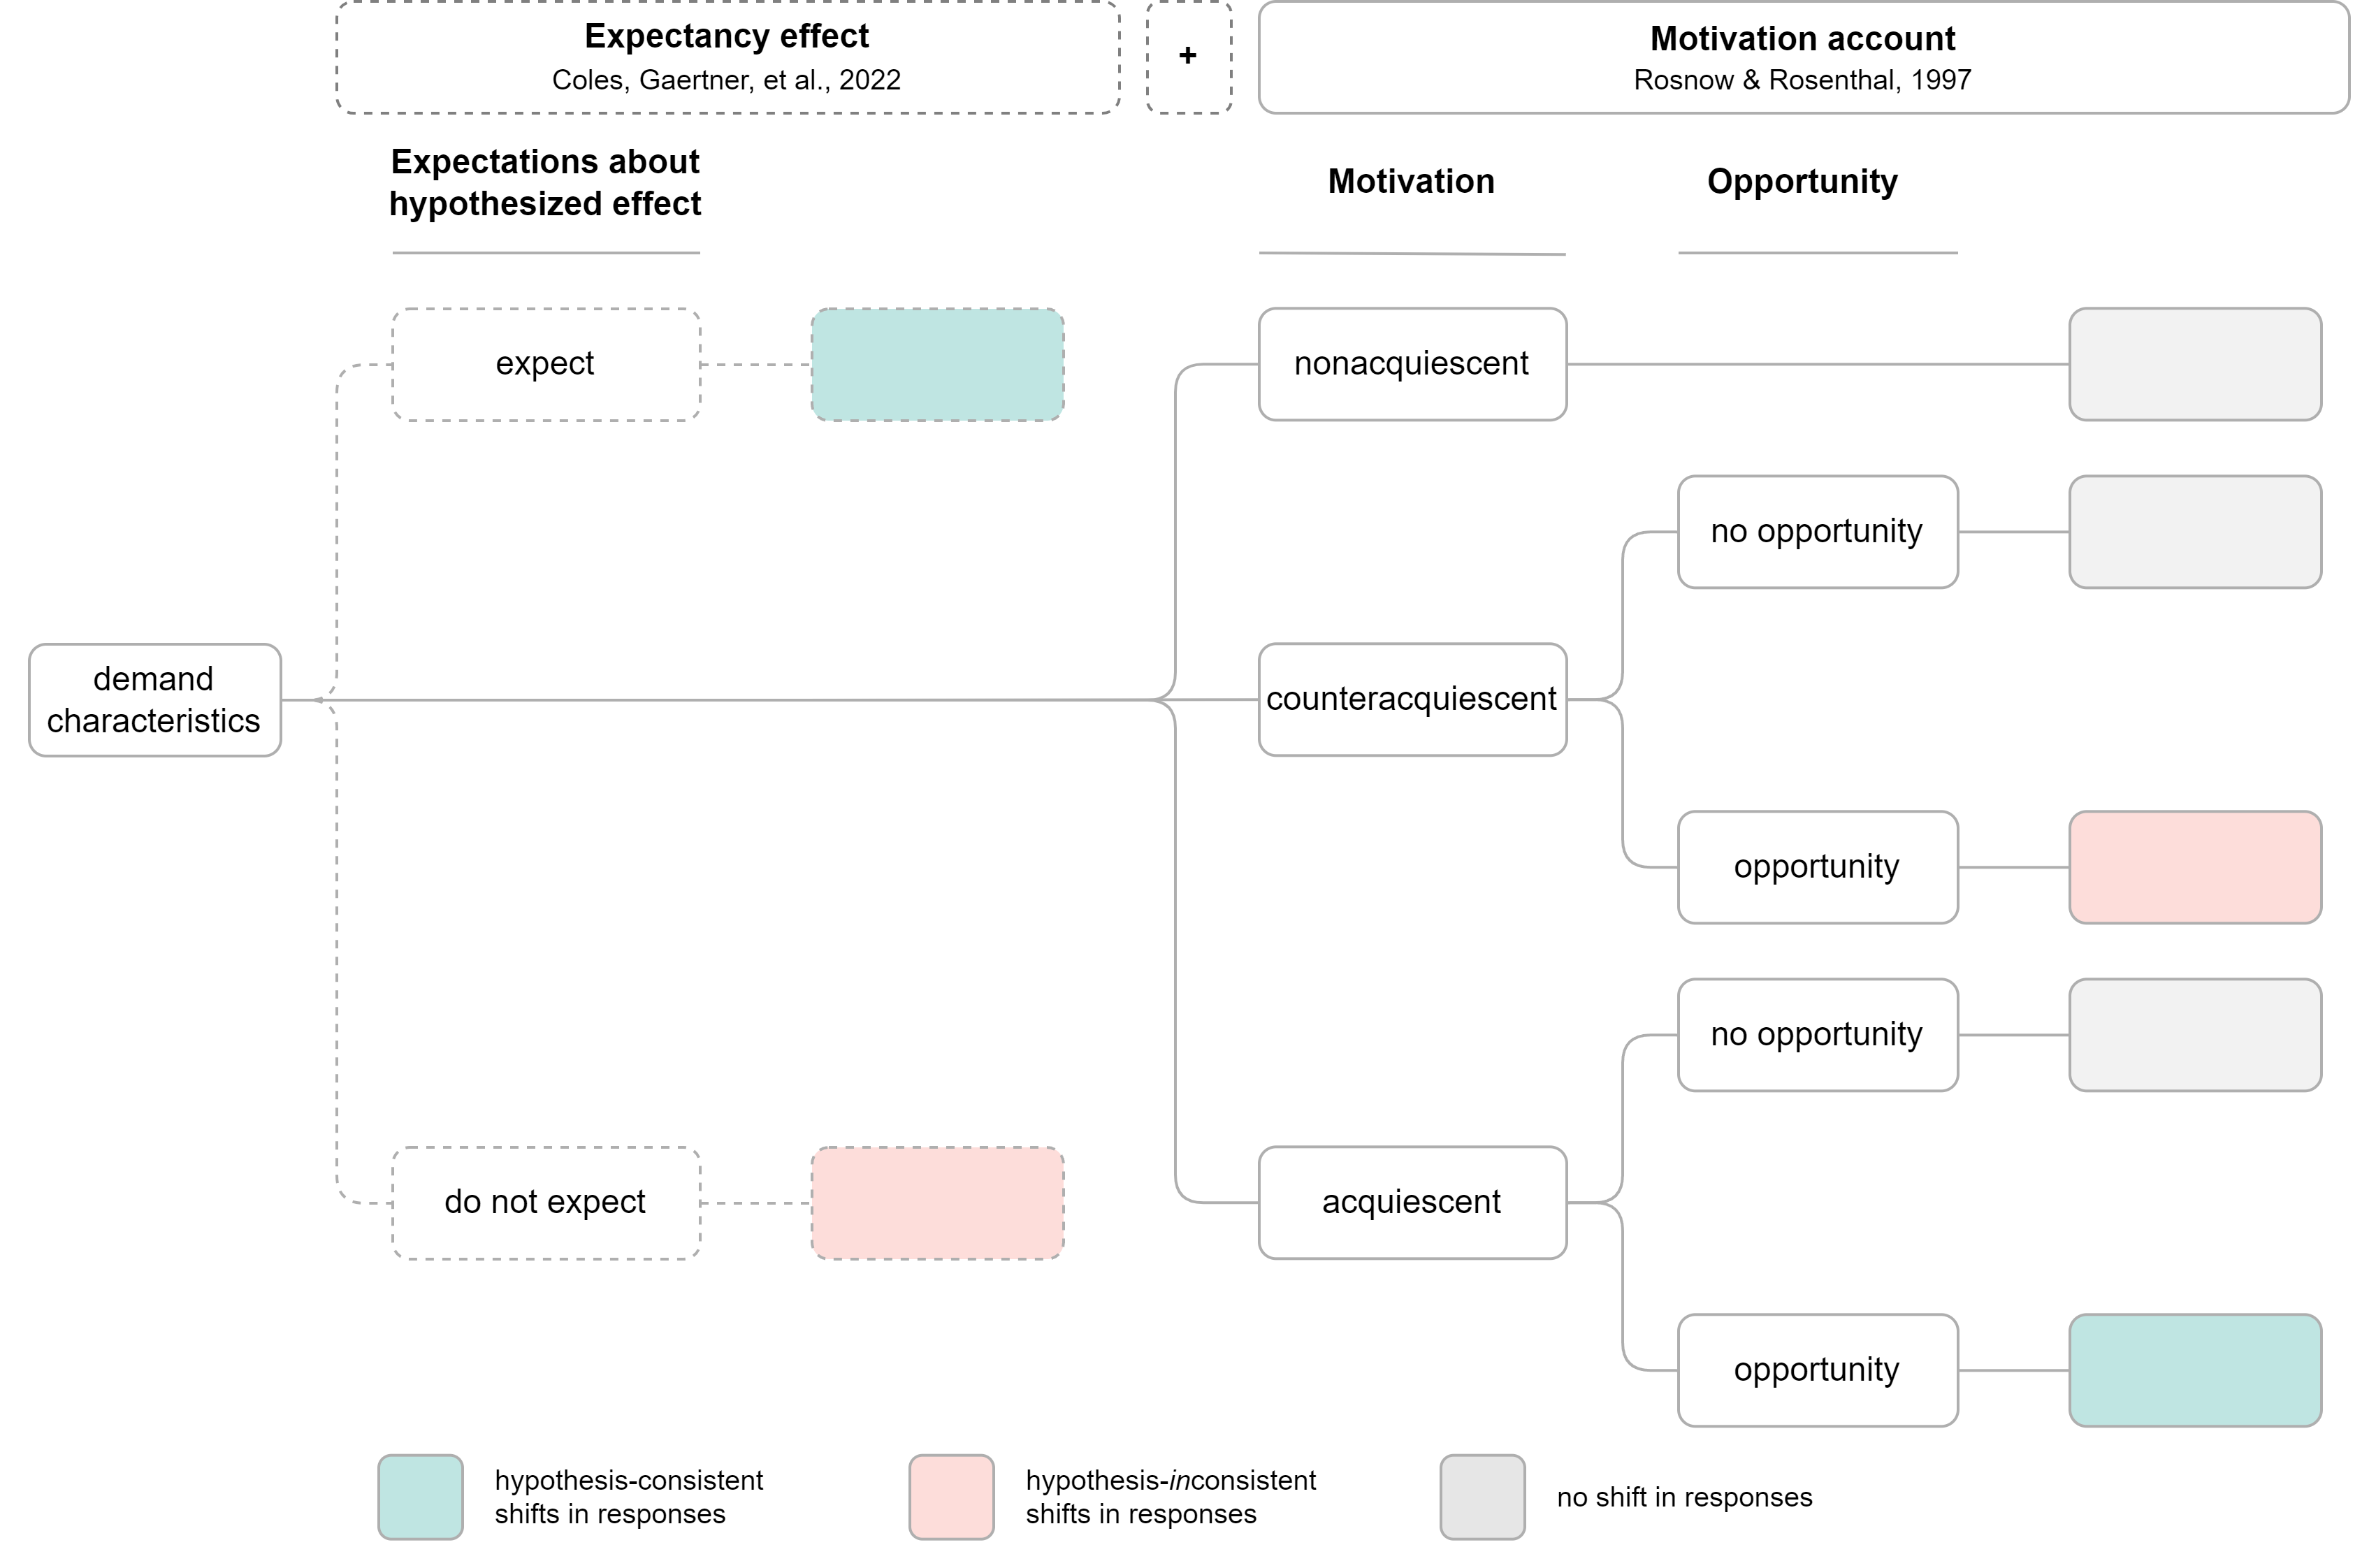
\includegraphics[width=11.35in]{images/metaware_framework} \caption{Rosnow and Rosenthal’s (1997) and Coles, Gaertner, et al.’s (2022) frameworks for conceptualizing how demand characteristics can lead to increases (green), decreases (red), or no shift (light grey) in hypothesis-consistent responding. Rosnow and Rosenthal conceptualized demand effects as response biases moderated by receptivity to cues (not pictured), motivation, and opportunity to adjust responses. Coles, Gaertner, et al. proposed that demand characteristics can also produce placebo biases (dotted boxes) that occur by activating or changing participants’ beliefs.}\label{fig:framework}
\end{figure}

To start, Rosnow and Rosenthal (1997) reasoned that participants must be perceptive to demand characteristics in order for there to be a response bias (see also Rosnow \& Aiken, 1973; Strohmetz, 2008). As an extreme example, imagine that a researcher hands an infant participant a sheet of paper that precisely explains the study hypothesis. Demand characteristics are certainly present, but they are not predicted to have an impact because the infant is not receptive to the cues. In the present work, we will pay less attention to receptivity as a moderator by focusing on scenarios where participants are likely to be highly receptive to cues.

Response biases are theorized to be driven by participants' motivation (or lack thereof) to provide hypothesis-consistent responses. Early research focused on participants' default motivations, characterizing them as (a) ``good subjects'' who change their responses because they are motivated to help the researcher confirm their hypothesis (Orne, 1962), (b) ``apprehensive subjects'' who are motivated to respond in a manner that will lead them to be evaluated positively (Riecken, 1962; Rosenberg, 1969; Sigall, Aronson, \& Van Hoose, 1970), (c) ``negativistic subjects'' who interfere with the purpose of the study (Cook et al., 1970; Masling, 1966), or (d) ``faithful subjects'' who attempt to follow directions as closely as possible (Fillenbaun \& Frey, 1970). However, participants have multiple goals in mind when they conceptualize their roles as subjects (Rosnow \& Rosenthal, 1997), and situational forces may affect which of these goals are most salient. For example, participants increase performance on simple tasks when told that this is the experimenter's expectation but not in contexts where the experimenter indicates that increased performance will be indicate of an obsessive-compulsive personality (Sigall et al., 1970).

Synthesizing the above observations and reasoning, Rosnow and Rosenthal (1997) suggested that, depending on the context, participants can be characterized as being overall motivated to either (a) non-acquiesce (i.e., not change their responses based on knowledge about the hypothesis), (b) acquiesce (i.e., provide hypothesis-consistent responses), or (c) counter-acquiesce (i.e., provide hypothesis-inconsistent responses). Of course, as we later discuss, motivation can also be conceptualized on a continuum ranging from highly motivated counter-acquiescence to highly motivated acquiescence.

No matter how motivated they are to confirm the hypothesis, there is variability in the extent to which participants have the opportunity/ability to alter the outcome of interest. For example, participants can more readily alter their responses to self-report measures of prejudice, as opposed to reaction-time-based measures like the Implicit Association Test (Greenwald, McGhee, \& Schwartz, 1998). Taking this third moderator -- opportunity -- into account, Rosnow and Rosenthal concluded that demand characteristics only produce response biases when participants (1) notice the cues, (2) are motivated to adjust their responses, and (3) can adjust their responses.

Rosenthal and Rosnow's framework directly maps onto psychologists' playbook for avoiding the impact of demand characteristics: use deception (reduce receptivity), incentivize honest reporting (reduce motivation), and/or deploy difficult-to-control outcome measures (reduce opportunity to adjust responses). However, we next turn our attention to a recently-proposed secondary mechanism that is more challenging to eliminate: placebo effects.

Over the past half century, demand characteristics have generally been conceptually divorced from placebo effects Rosnow \& Rosenthal (1997). However, demand characteristics may produce both response biases and \emph{placebo effects} mediated by the relatively automatic activation of beliefs and/or conditioned responses Corneille \& Lush (2022). For example, after inferring that a researcher expects an intervention to boost mood, a participant may both (a) deliberately adjust their mood ratings (a response bias), and (b) unintentionally experience a placebo-induced change in mood. Consistent with this reasoning, Coles, Gaertner, et al. (2022) found that participants' beliefs about facial feedback effects did not always match the hypothesis communicated; furthermore, both the communicated hypothesis and measures of participants' beliefs moderated the effects of posed expressions on emotion. This finding provides preliminary evidence that demand characteristics can produce both response biases and placebo effects, meaning that demand characteristics can still bias responses when participants have neither the motivation nor the opportunity to adjust their responses.

\hypertarget{the-current-paper}{%
\subsection{The current paper}\label{the-current-paper}}

The goal of the current paper is to take stock of what we know about demand characteristics as a methodological artifact. In Study 1, we report a meta-analysis of strict experimental tests of the effects of demand characteristics. We then examine several study features (e.g., whether participants are paid) that may moderate these effects.

In Study 2, we report an extension of the meta-analysis that examines whether observed effect size variability can be explained by factors theorized to underlie response biases (i.e., motivation and opportunity to adjust responses) and placebo effects (i.e., belief in the experimenter's hypothesis). To conduct this moderation analysis, we derived estimates of these factors from a new set of participants. These participants read descriptions of each study in the meta-analysis and then reported the extent to which they hypothetically would have (a) been motivated to confirm the experimenter's hypothesis, (b) had the opportunity to adjust their responses, and (c) believed the experimenter's hypothesis. We also examined how well this new set of participants could predict the effects of the studies' demand characteristic manipulations.

In Study 3, we report a replication experiment that re-examines the extent to which demand effects are driven by response biases and placebo effects. In this replication study, we manipulated demand characteristics in an experiment on the proposed effects of facial poses on emotional experience (Coles, Larsen, \& Lench, 2019; Coles, March, et al., 2022). We then examined the extent to which the effect of facial poses was moderated by the factors believed to underlie response biases and placebo effects.

\hypertarget{study-1}{%
\section{Study 1}\label{study-1}}

Study 1 was designed to provide a quantitative synthesis of demand effects via meta-analysis.

\hypertarget{methodology}{%
\subsection{Methodology}\label{methodology}}

We defined the scope of the meta-analysis using the Population, Intervention, Comparison, Outcome framework (Schardt, Adams, Owens, Keitz, \& Fontelo, 2007). Our population-of-interest was human subjects participating in non-clinical studies. We excluded clinical studies so that we could focus on research that better isolates the discipline (experimental psychology) and mechanism (response bias) most often discussed in the demand characteristics literature. Given that there is a sizable literature on placebo effects, excluding clinical studies improved the feasibility of the meta-analysis.

The intervention-of-interest was explicit manipulations of the hypothesis communicated to participants -- i.e., scenarios where a researcher tells participants about the effect of an independent variable on a dependent variable. Demand characteristics are sometimes defined as \emph{any} cue that may impact participants' beliefs about the purpose of the study, including instructions, rumors, and experimenter behavior (Orne, 1962). However, such a definition creates a blurry and potentially boundless conceptual space where any systematic change in a research design might be considered a test of demand characteristics. To bound and simplify the conceptual space, we focused on explicit manipulations of the hypothesis communicated to participants.

Our comparison-of-interest were conditions where either no hypothesis or a different hypothesis was communicated to participants. Our outcome-of-interest was the dependent variable described in the communicated hypothesis. For example, in a study that manipulated whether the intervention is described as ``mood-boosting'', the outcome-of-interest would be any measure of mood.

\hypertarget{literature-search}{%
\subsubsection{Literature search}\label{literature-search}}

Our literature search strategy was developed in consultation with a librarian at Stanford University. Given the broad nature of the demand characteristics construct, we determined that a truly comprehensive strategy was not feasible. Thus, we sought to design a strategy that best balanced comprehensiveness and feasibility.

We searched APA PsycInfo using broad search terms: ``demand characteristics'' OR ``hypothesis awareness''. This yielded 850 records. We also released a call for unpublished studies on the Society for Personality and Social Psychology Open Forum; Twitter; the Facebook Psychological Methods Discussion group; and the Facebook PsychMAP group. This yielded 3 additional records. In total, 97 of the records were unpublished.

\hypertarget{screening}{%
\subsubsection{Screening}\label{screening}}

To be eligible for inclusion in the meta-analysis, the following criteria must have been met:

\begin{itemize}
\item
  The researcher manipulated what participants were told about the effect of an independent variable on a dependent variable. This included both \emph{positive demand} (participants told that the dependent variable will increase), \emph{negative demand} (participants told that the dependent variable will decrease) and \emph{nil demand} (participants told the dependent variable will be unaffected) conditions. Often, this was compared to a \emph{control} condition, where participants were not told about an effect of an independent variable on a dependent variable.\footnote{We excluded conditions where the researcher communicated a \emph{non-directional} effect. We did so because participants in these scenarios could not unambiguously infer how their responses were expected to change. For example, if participants were told that an independent variable would ``impact mood'', it is not clear if participants should infer that the mood will be boosted or dampened.}
\item
  The demand characteristics manipulation was not strongly confounded. For example, we excluded a study by Sigall et al. (1970) because the manipulation of the stated hypothesis was confounded with a disclosure about the meaning of the behavior (i.e., that confirming the hypothesis would be indicative of an obsessive-compulsive personality disorder).
\item
  Information necessary for computing at least one effect size was included.
\end{itemize}

N. C. and a research assistant screened records independently, reviewed potentially relevant records together, and worked together to code the information for moderator analyses and effect size computations. Disagreements and discrepancies were resolved through discussion. In total, 42 studies from 31 records were eligible for inclusion. However, one record (Allen \& Smith, 2012) was removed because the information provided led to implausibly large effect size estimates (e.g., \(d\) = -212.57).

\hypertarget{effect-size-index}{%
\subsubsection{Effect size index}\label{effect-size-index}}

We used standardized mean difference scores (Cohen's \(d_{s}\) and \(d_{rm}\)) as our effect size index (Borenstein, 2009; Cohen, 2013).

In most scenarios, we estimated the main effect of demand characteristics. For example, Coles, Gaertner, et al. (2022) manipulated whether participants were told that posing smiles would increase happiness. Here, the main effect of demand characteristics can be computed by comparing happiness ratings from smiling participants who were either informed or not informed of the mood-boosting effect of smiling.

In some scenarios, we estimated the \emph{interactive} effect of demand characteristics. For example, in the same Coles, Gaertner, et al. (2022) study, participants provided happiness ratings both after smiling and scowling. Participants' mood generally improved when smiling vs.~scowling (i.e., there was a main effect of facial pose). However, the difference was more pronounced when participants were told about the mood-boosting effects of smiling. In other words, there was an interaction between facial pose and demand characteristics. In this scenario, the interactive effect of demand characteristics was computed by calculating a standardized difference-in-differences score. These scores were computed similar to Cohen's \(d_{s}\) and \(d_{rm}\), but with mean-difference scores (as opposed to means).

Effect sizes were calculated so that positive values indicated an effect consistent with the communicated hypothesis. For example, if participants were told that an intervention should be mood boosting, an increase in mood would be coded as a positive effect. If, however, participants were told that the intervention should be mood \emph{dampening}, that same increase in mood would be coded as a negative effect.

Whenever possible, we used the \emph{M}'s and \emph{SD}'s reported in a paper to compute Cohen's \emph{d}. If these values were not reported, we used (in order of preference), (1) \emph{t}-values, (2) descriptive statistics extracted from figures (e.g, bar charts) using the WebPlotDigitizer (Drevon, Fursa, \& Malcolm, 2017), (3) \emph{F}-values, or (4) \emph{p}-values. In instances where this information was not provided but the significance and direction of the effect was described, we assumed \emph{p}-values of .04 and .50 for significant and non-significant effects respectively (e.g., Kenealy, 1988). In a few instances, the outcome variable in a study was discrete (as opposed to continuous). In these cases, we approximated a Cohen's \emph{d} score based on a transformation of the log odds ratio (Borenstein, Hedges, Higgins, \& Rothstein, 2011).

For repeated-measure comparisons, the correlation between the repeated measures is needed to calculate Cohen's \(d_{rm}\). This correlation is rarely reported, so we followed a recommendation by Borenstein (2009) and performed sensitivity analyses on an assumed correlation. We preregistered a default correlation of \(r\) = .50 but performed sensitivity analysis with \(r\) = .10, .30, .50, .70, and .90. These sensitivity analyses produced virtually no change in overall effect size estimates, so we do not discuss them further.

Nearly all studies (85\%) contained multiple effect sizes of interest. For example, the full design in Coles, Gaertner, et al. (2022) included a positive demand, nil demand, and control condition. Participants also completed several facial expression poses (happy, angry, and neutral) and self-reported several emotions (happiness and anger). To be comprehensive, we recorded all reported effect sizes and accounted for dependencies in our models (described later).

\hypertarget{potential-study-feature-moderators}{%
\subsubsection{Potential study feature moderators}\label{potential-study-feature-moderators}}

We coded several study feature moderators that may help explain variability in demand effects:

\begin{itemize}
\item
  \emph{Control vs.~non-control group comparison group}. Demand effects should presumably be additive. For example, imagine a study where the effect of an task is either (a) not described at all (a control condition), (b) described as mood-boosting (positive demand) or (c) described as mood-dampening. Compared to the control condition, mood is typically predicted to be boosted in the positive demand condition and dampened in the negative demand condition. If this is the case, the mean difference in mood should be larger when the positive demand condition is compared to the negative demand condition (as opposed to the control condition). To test this, we coded whether comparisons were made to a control group or a different demand condition.
\item
  \emph{Positive, negative, or nil demand.} Instances where a demand characteristic condition was compared to a control group allowed us to additionally test whether participants responses shift more when the researcher hypothesizes an increase in the dependent variable (positive demand), a decrease (negative demand), or no change in the dependent variable (nil demand).
\item
  Whether students, non-students (e.g., MTurk workers), or a mix of students and non-students were sampled.
\item
  Whether the study was conducted online or in-person.
\item
  Whether demand characteristics were manipulation within- vs.~between-subjects.
\item
  Whether participants were paid or unpaid.
\end{itemize}

\hypertarget{meta-analytic-approach}{%
\subsubsection{Meta-analytic approach}\label{meta-analytic-approach}}

We used three-level meta-analysis (3LMA; also referred to as ``multilevel'' meta-analysis), which accommodates nested effect sizes by modeling three sources of variability: sampling error of individual studies (level 1), variability within studies (level 2), and variability between studies (level 3; often referred to as ``random effects''). To estimate the overall effect size, we fit an intercept-only 3LMA model. Unless otherwise specified, we conducted moderator analyses by separately entering dummy-coded categorical factors, which were used to estimate the moderating relationship and the effect size within each subgroup of the moderator. Our pre-registration plan and documented amendments are available at \url{https://osf.io/3hkre/}.

\hypertarget{publication-bias-analyses}{%
\paragraph{Publication bias analyses}\label{publication-bias-analyses}}

Publication bias refers to the well-documented propensity for hypothesis-inconsistent findings to be disproportionately omitted from the published scientific record (Franco, Malhotra, \& Simonovits, 2014). When present, publication bias can lead to inaccurate effect size estimates and inferential errors in meta-analysis. Consequently, we used three main approaches for assessing and correcting for potential publication bias in our estimation of the overall effect of demand characteristics.

First, we visually examined \emph{funnel plots,} wherein observed effect sizes are plotted against a measure of their precision (e.g., standard error). In the absence of publication bias, the distribution typically resembles a funnel; relatively large studies estimate the effect with high precision, and effect sizes fan out in \emph{both} directions as the studies become smaller. If, however, non-significant findings are disproportionately omitted from the scientific record (i.e., there is publication bias), the distribution is often asymmetric/sloped. Funnel plots traditionally contain one effect size per study, but many of our studies produced multiple effect sizes. Thus, we examined two funnel plots: one with all effect sizes and one with the dependent effect sizes aggregated\footnote{For effect size aggregation, we assumed a default dependent effect size correlation of \(r\) = .50 but performed sensitivity analysis with \(r\) = .10, .30, .50, .70, and .90. These sensitivity analyses did not change our overall conclusion about publication bias, so we do not discuss them further.}.

Second, we conducted precision-effect tests (Stanley \& Doucouliagos, 2014). In precision-effect tests, the relationship between observed effect sizes and their standard errors -- which is typically absent when there is no publication bias -- is estimated and controlled for in a meta-regression model. The slope of this model is generally interpreted as an estimate of publication bias, and the intercept is interpreted as the bias-corrected overall effect. Precision-effect tests were developed and validated for meta-analyses with independent effect sizes. Nonetheless, Rodgers and Pustejovsky (2021) demonstrated that the method retains fairly good statistical properties when (1) 3LMA is used or (2) dependent effect sizes are aggregated and modeled using random-effects (i.e., two level) meta-regression. We used both approaches.

Third, we used weight-function modeling (Vevea \& Hedges, 1995). In weight-function modeling, weighted distribution theory is used to model biased selection based on the significance of observed effects. If the adjusted model provides increased fit, publication bias is a concern and the model can be used to estimate the bias-corrected overall effect size. Once again, weight-function modeling was designed for independent effect sizes. Nonetheless, it has fairly good statistical properties when non-independent effect sizes are aggregated, which we did here (Rodgers \& Pustejovsky, 2021).

As a sensitivity analysis, we included publication status (published or unpublished) as a dummy-coded predictor to our overall-effect 3LMA. This allowed us to estimate the difference in the magnitude of published vs.~unpublished effects.

\hypertarget{results}{%
\subsection{Results}\label{results}}

Overall, explicit manipulations of demand characteristics cause participants' responses to shift in a manner consistent with the communicated hypothesis, \(d\) = 0.22, 95\% CI {[}0.11, 0.33{]}, \(t\) = 3.93, \(p\) \textless{} .001. As a hypothetical example, if participants were told that the researcher hypothesizes that an intervention will improve mood (positive demand), they would generally report slightly improved moods; if told that the researcher hypothesizes that an intervention will worsen mood (negative demand), they would generally report slightly worsened moods.

\begin{figure}
\centering
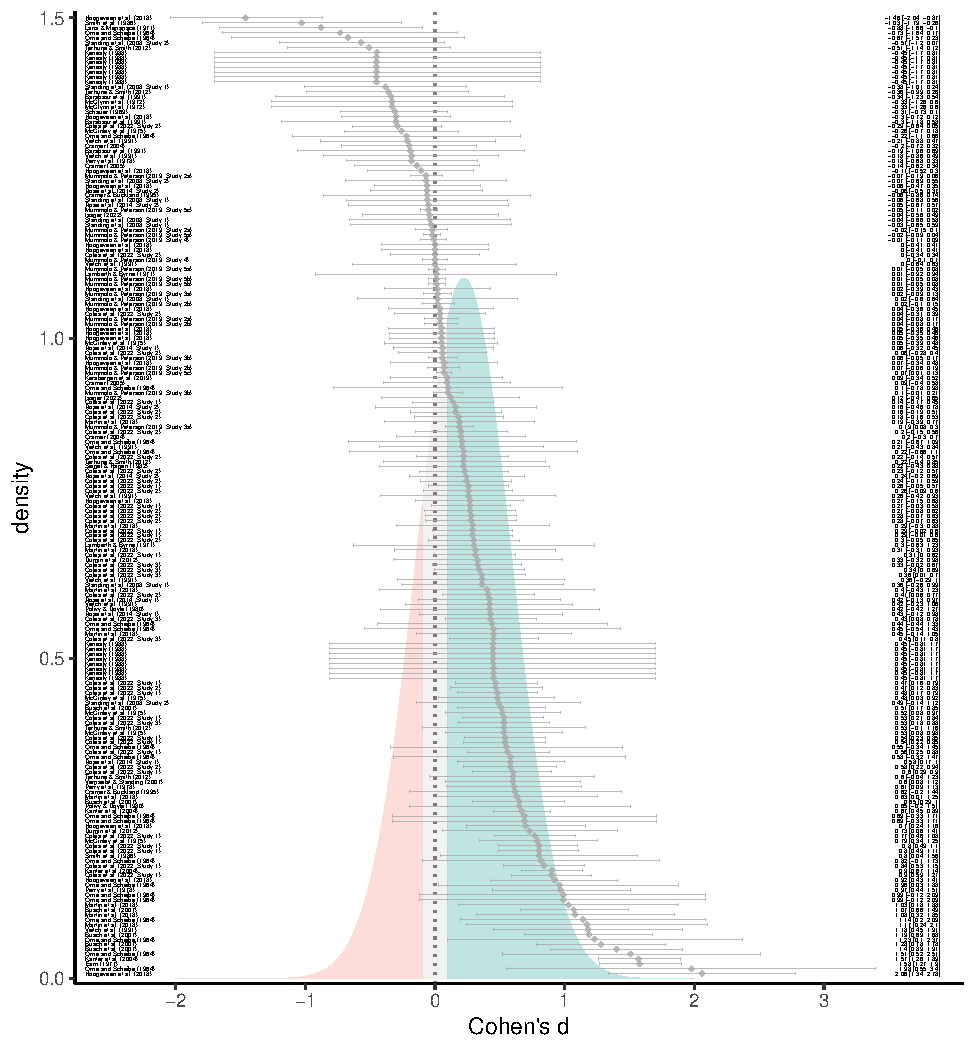
\includegraphics{metaware_manuscript_files/figure-latex/forest-1.pdf}
\caption{\label{fig:forest}Forest plot of estimated effect sizes (grey diamonds), their 95\% confidence intervals (grey error bars), and their citations (left). The estimated effect size distribution is also shown and colored based on whether demand characteristics produce more hypothesis-consistent responding (green; d \textgreater{} 0.10), more hypothesis-inconsistent responding (red; d \textless{} -0.10), or negligible shifts in responding (grey; \textbar d\textbar{} \textless{} 0.10).}
\end{figure}

Although demand characteristics produce more hypothesis-consistent responding \emph{on average}, these effects are not consistent (between-study \(\tau\) = 0.30; within-study \(\sigma\) = 0.20; Figure \ref{fig:forest}). Based on the meta-analytic mean and standard deviation (between-study \(\tau\) + within-study \(\sigma\)), we estimated that \emph{true} demand effects can range from approximately \(d\) = -1.48 to \(d\) = 2.10. For the sake of example, we arbitrarily classified any effect size less than 0.10 standard deviation in either direction as ``negligible''. Based on this classification, our results indicate that demand characteristics most often produce hypothesis-consistent shifts (63\%), but sometimes produce negligible shifts (18\%) or shifts in the \emph{opposite} direction of the communicated hypothesis (19\%).

\hypertarget{moderator-analyses}{%
\subsubsection{Moderator analyses}\label{moderator-analyses}}

\begin{figure}
\centering
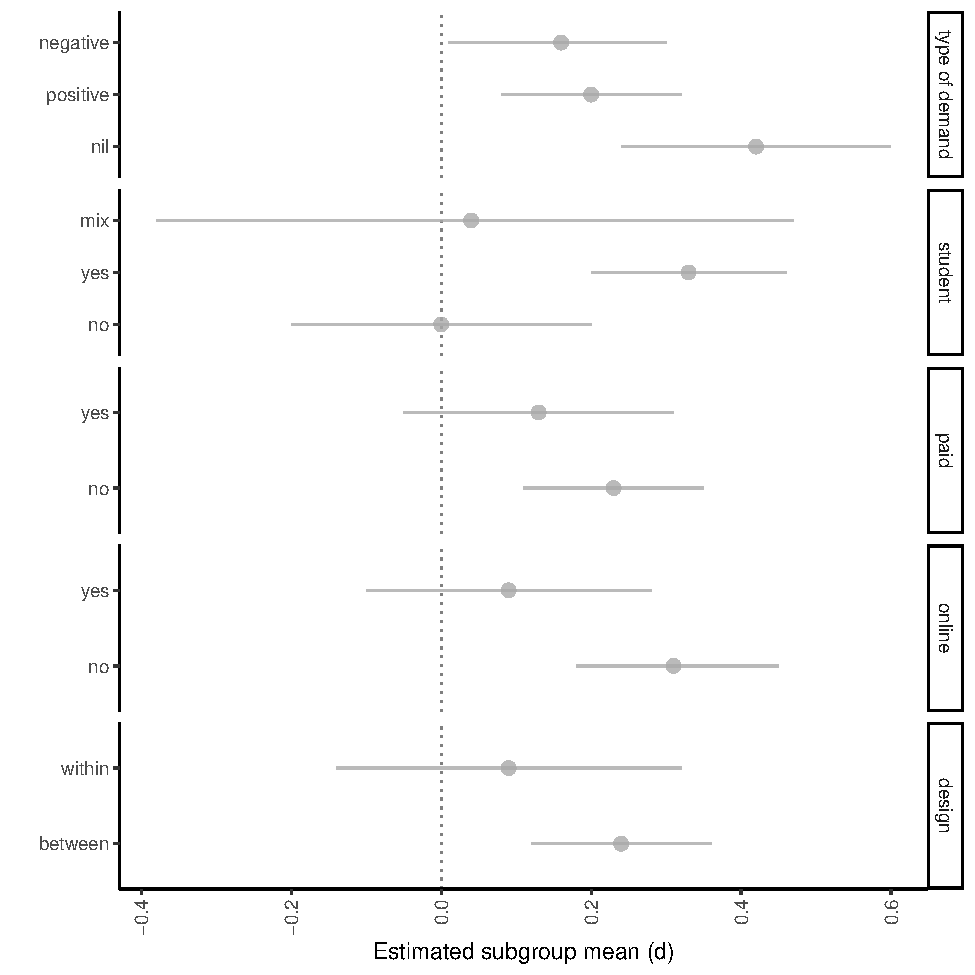
\includegraphics{metaware_manuscript_files/figure-latex/modforest-1.pdf}
\caption{\label{fig:modforest}Selected moderator subgroup mean effect sizes (dots) and their 95\% confidence intervals (error bars).}
\end{figure}

The observed variability in demand effects dramatically exceeded what would be expected from sampling error alone, \(Q\)(194) = 901.77, \(p\) \textless{} .001. This heterogeneity suggests the existence of moderators.

The effects of demand characteristics tended to differ by participant pool, \(F\)(2, 182) = 4.12, \(p\) = .018. As shown in Figure \ref{fig:modforest}, effects were generally positive and medium-to-large in studies with students (\(d\) = 0.33, 95\% CI {[}0.20, 0.46{]}, \(p\) \textless{} .001), and near-zero in studies with non-students (\(d\) = 0.00, 95\% CI {[}-0.20, 0.20{]}, \(p\) = .993) or a mix of students and non-students (\(d\) = 0.04, 95\% CI {[}-0.38, 0.47{]}, \(p\) = .838). The effects of demand characteristics also tended to be slightly more positive for in-person (\(d\) = 0.31, 95\% CI {[}0.18, 0.45{]}, \(p\) \textless{} .001) vs.~online (\(d\) = 0.09, 95\% CI {[}-0.10, 0.28{]}, \(p\) = .373) studies, but this difference was not significant, \(F\)(1, 189) = 3.61, \(p\) = .059 (Figure \ref{fig:modforest}).

The effects of demand characteristics appeared to be additive. Compared to instances where a demand characteristic condition was compared to a control group (\(d\) = 0.16, 95\% CI {[}0.04, 0.28{]}, \(p\) = .009), effect sizes were approximately twice as large when two demand characteristic conditions were compared (\(d\) = 0.37, 95\% CI {[}0.24, 0.51{]}, \(p\) \textless{} .001), \(F\)(1, 193) = 19.26, \(p\) \textless{} .001. Instances where a demand characteristic condition was compared to a control group allowed us to additional test whether participants respond more strongly to positive, nil, or negative demand characteristics. Results indicated that they might, \(F\)(2, 131) = 5.41, \(p\) = .006. As shown in Figure \ref{fig:modforest}, the effect of demand characteristics tended to be nearly twice as large in the nil (\(d\) = 0.42, 95\% CI {[}0.24, 0.60{]}, \(p\) \textless{} .001) vs.~positive (\(d\) = 0.20, 95\% CI {[}0.08, 0.32{]}, \(p\) = .002), and negative demand conditions (\(d\) = 0.16, 95\% CI {[}0.01, 0.30{]}, \(p\) = .034). In other words, participants' responses most strongly shifted when researchers communicated that \emph{no} effect is expected.

We did not find that the effects of demand characteristics tended to differ depending on whether they were manipulated within- (\(d\) = 0.24, 95\% CI {[}0.12, 0.36{]}, \(p\) \textless{} .001) vs.~between-subjects (\(d\) = 0.09, 95\% CI {[}-0.14, 0.32{]}, \(p\) = .427), \(F\)(1, 193) = 1.66, \(p\) = .199 (Figure \ref{fig:modforest}. We also did not find that the effects of demand characteristics differed by the year the record was completed or published, \(\beta\) = 0.00, 95\% CI {[}-0.01, 0.00{]}, \(t\)(194) = -0.51, \(p\) = .607.

The effects of demand characteristics tended to be \emph{numerically} larger in unpaid (\(d\) = 0.23, 95\% CI {[}0.11, 0.35{]}, \(p\) \textless{} .001) vs.~paid (\(d\) = 0.13, 95\% CI {[}-0.05, 0.31{]}, \(p\) = .157) studies -- but this difference was not statistically significant, \(F\)(1, 192) = 0.87, \(p\) = .352 (Figure \ref{fig:modforest}).

\hypertarget{exploratory-robustness-checks}{%
\subsubsection{Exploratory robustness checks}\label{exploratory-robustness-checks}}

The above moderator analyses indicated that demand characteristics tend to produce larger increases in hypothesis-consistent responding when students are sampled, studies are run in-person, and participants are uncompensated. However, an exploratory inspection of the data revealed that these variables are correlated. For example, effect size estimates were more likely to be based on student samples for in-person (82\%) vs.~online (59\%) studies. Effect size estimates were also more likely to be based on student samples for unpaid (83\%) vs.~paid (53\%) studies.

As an exploratory robustness check, we fit a 3LMA with student status, data collection medium, and payment status entered as effect-coded factors. This exploratory analysis indicated that student status -- but not data collection medium (\emph{F}(1, 175) = 0.18, \emph{p} = .669) or payment status (\emph{F}(1, 175) = 1.18, \emph{p} = .280) -- was a significant moderator of demand effects, \emph{F}(2, 175) = 3.44, \emph{p} = .034. In other words, only student status was robustly associated with differences in demand effects in a more complex model.

\hypertarget{estimating-demand-effects-in-specific-study-contexts}{%
\subsubsection{Estimating demand effects in specific study contexts}\label{estimating-demand-effects-in-specific-study-contexts}}

\begin{figure}
\centering
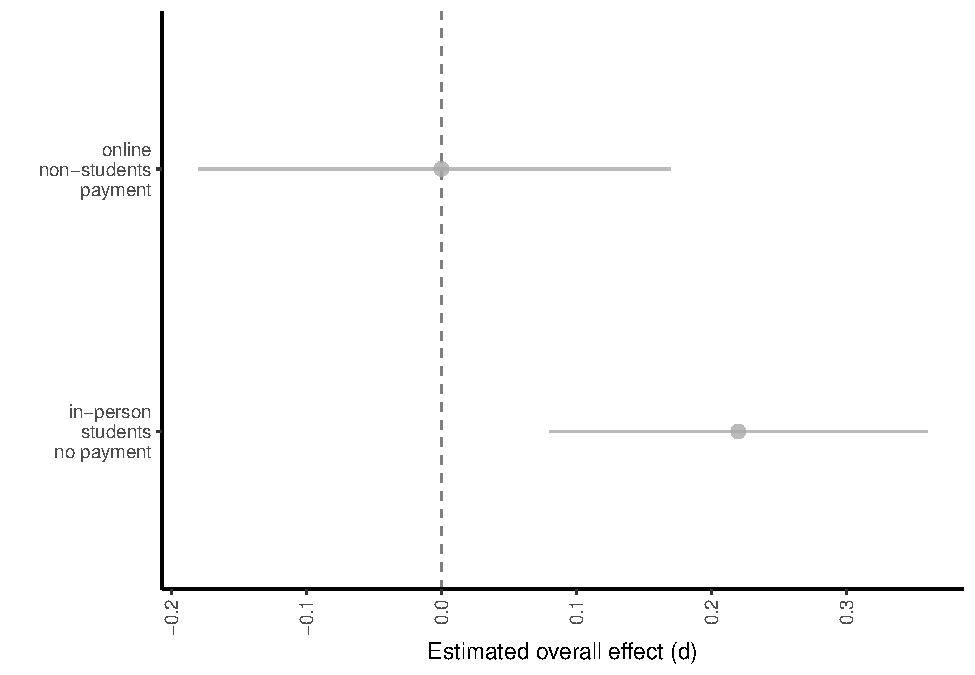
\includegraphics{metaware_manuscript_files/figure-latex/predplot-1.pdf}
\caption{\label{fig:predplot}Estimated overall effect of positive demand characteristics in a classic experimental setting (in-person study testing a positive effect with a volunteer student sample) and an online worker setting (online study testing a positive effects with a paid non-student sample)}
\end{figure}

Our models allow estimation of the effects of demand characteristics in various study contexts. To explore this functionality (and to demonstrate a potentially use for our dataset in the future), we fit a 3LMA with student status, data collection medium, payment status, and type of demand characteristic comparison entered as dummy-coded factors. By changing the reference level of these dummy-coded factors, we were able to derive estimates of demand effects in two common scenarios described below.

First, we estimated the overall impact of demand characteristics in what we call a ``classic experimental setting'': studies that (a) are run in-person, (b) sample students, (c) do not offer participant payment, and (d) are testing for a positive effect (i.e., positive demand). In this context, overt demand characteristics are estimated to typically produce a small increase in hypothesis-consistent responding, \(d\) = 0.22, 95\% CI {[}0.08, 0.36, \(p\) = .003{]} (Figure @ref(fig:predictions\_plot)). Second, we estimated the overall impact of demand characteristics in an an ``online worker experimental context'': studies that (a) are run online, (b) sample non-students, (c) offer participant payment, and (d) are testing for a positive effect Here, we did not find that demand characteristics, on average, produce changes in participants' responses, \(d\) = 0.00, 95\% CI {[}-0.18, 0.17, \(p\) = 0.97{]} (Figure \ref{fig:predplot}).

\hypertarget{publication-bias-analyses-1}{%
\subsubsection{Publication bias analyses}\label{publication-bias-analyses-1}}

Overall, publication bias analyses were inconclusive. A funnel plot containing all effect sizes appeared to indicate that publication bias favored instances where participants' responses shifted in a hypothesis-consistent manner. However, a funnel plot where non-independent effect sizes were aggregated appeared to indicate the opposite: that publication bias favored non-significant or hypothesis-inconsistent shifts in participants' responses.

Precision-effect tests similarly yielded opposite conclusions depending on whether we used (a) 3LMA with non-aggregated effect size estimates, or (b) two-level meta-analysis with aggregated dependent effect size estimates. On one hand, precision-effect tests with 3LMA provided a non-significant estimate of publication bias that favored hypothesis-consistent shifts in participants' responses, \(\beta\) = 0.68, 95\% CI {[}-0.07, 1.44{]}, \(p\) = .076. The bias-corrected overall effect size estimate did not significantly differ from zero, \(d\) = 0.06, 95\% CI {[}-0.16, 0.27{]}, \(p\) = .606. On the other hand, two-level precision-effect tests with aggregated dependent effect size estimates yielded an opposite pattern: that there was a slight (but not statistically significant) preference for non-significant or hypothesis-inconsistent shifts in participants' responses, \(\beta\) = -0.34, 95\% CI {[}-1.39, 0.70{]}, \(p\) = .519. The bias-corrected overall effect size estimate was thus slightly adjusted upward, \(d\) = 0.23, 95\% CI {[}0.01, 0.45{]}, \(p\) = .038. In other words, depending on how dependencies were handled, precision-effect tests yielded inconsistent conclusions about the direction of publication bias and the significance of the bias-corrected overall effect of demand characteristics.

A weight-function model suggested that better fit was achieved with a model indicating that publication bias favored non-significant or hypothesis-inconsistent shifts in participants' responses, \(\chi^2\)(1) = 10.80, \(p\) = .001. The bias-corrected overall effect size was thus upward-adjusted, \(d\) = 0.41, 95\% CI {[}0.19, 0.62{]}, \(p\) \textless{} .001. A comparison of unpublished (\(d\) = 0.46, 95\% CI {[}0.00, 0.91{]}, \(p\) = .050) and published (\(d\) = 0.21, 95\% CI {[}0.09, 0.32{]}, \(p\) \textless{} .001) studies yielded a similar pattern, although the difference was not significant, \(F\)(1, 193) = 1.08, \(p\) = .301.

\begin{figure}
\centering
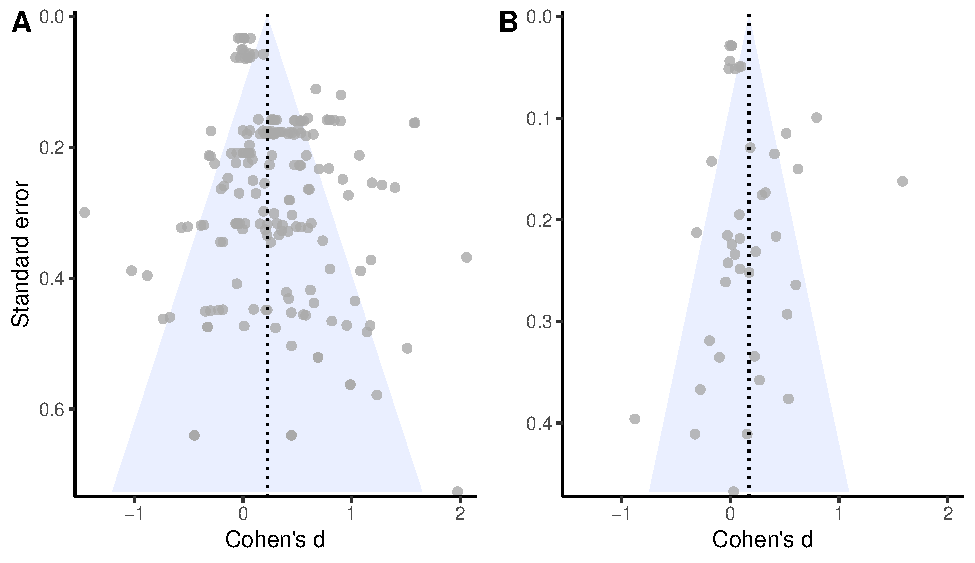
\includegraphics{metaware_manuscript_files/figure-latex/funnel-1.pdf}
\caption{\label{fig:funnel}Raw (A) or aggregated (B) effect sizes plotted against their corresponding standard errors.}
\end{figure}

\hypertarget{discussion}{%
\subsection{Discussion}\label{discussion}}

Overall, explicit manipulations of demand characteristics caused participants' responses to shift in a manner consistent with the communicated hypothesis. However, effects were very heterogeneous. As an illustration, we estimated that 63\% of demand characteristics manipulations produce hypothesis-consistent shifts (\(d\) \textgreater{} 0.10), 19\% produce hypothesis-\emph{in}consistent shifts (\(d\) \textless{} -0.10), and 18\% produce negligible shifts in either direction (-0.10 \textless{} \(d\) \textgreater{} 0.10). Moderator analyses revealed three study features that were associated with more hypothesis-consistent shifts in responses: (1) sampling student populations, (2) running studies in-person, and (3) communicating that the researchers hypothesizes there will be \emph{no} shift in responses (i.e., using nil demand manipulations). Of the three, sampling student populations appeared the be the most robust moderator.

Practically speaking, we estimated that demand characteristics are predicted to produce small increases in hypothesis-consistent responding in ``classic experimental settings'' (in-person studies testing a positive effect with unpaid student subjects). In contrast, when these studies are run online with paid workers -- an ``online worker experimental setting'' -- we estimated that demand effects are near zero. However, these results are ultimately preliminary given the high heterogeneity and inconsistent evidence of the direction and impact of publication bias.

Study 1 provides preliminary insights on the magnitude, consistency, and contextual moderators of demand effects. However, it was not designed to evaluate outstanding questions regarding the extent to which these effects are driven by response bias and placebo effects. For example, consider our finding that demand characteristics tend to produce more hypothesis-consistent shifts in responses when students (vs.~workers) are sampled. If this is true, it may occur because students are more motivated to help the experimenter confirm their hypothesis (a response bias). Alternatively, it may occur because students are more likely to \emph{believe} the communicated hypothesis (a placebo effect). In other words, although we have preliminary evidence of contextual modifiers of demand effects, we still lack an explanation of why these contexts matter and how demand effects work more broadly. In Study 2, we begin investigating this outstanding issue through an extension of the meta-analysis.

\hypertarget{study-2}{%
\section{Study 2}\label{study-2}}

Study 2 was designed to examine whether observed variability in effect sizes can be explained by factors theorized to underlie response biases (i.e., motivation and opportunity to adjust responses) and placebo effects (i.e., belief in the experimenter's hypothesis; Figure \ref{fig:framework}). Unfortunately, these factors were rarely measured in the studies included in the meta-analysis. We thus estimated their values through an experiment.

Our rationale was that the best way to understand these factors would be to elicit judgments about their presence from na:ive participants. Using these measurements, we then tested their moderating role by entering the values into meta-regressions. Also through meta-regression, we examined whether a new set of participants could retroactively predict the effects of the demand characteristic manipulations in the Study 1 meta-analysis.

\hypertarget{methodology-1}{%
\subsection{Methodology}\label{methodology-1}}

For each study in the meta-analysis, we created vignettes that described the key details for each demand characteristic condition and dependent variable combination. For example, Standing, Verpaelst, and Ulmer (2008) had two demand characteristic manipulations (positive and negative demand) and two dependent variables (measures of verbal and spatial reasoning). Thus, we created four vignettes for this study (see Figure \ref{fig:vig}).

In total, there were 119 vignettes. We did not create vignettes for control conditions because participants were not given information about the experimenter's hypothesis. Because there were no explicit demand characteristics to act upon, we left motivation, belief, and opportunity values blank for this condition.

\begin{figure}
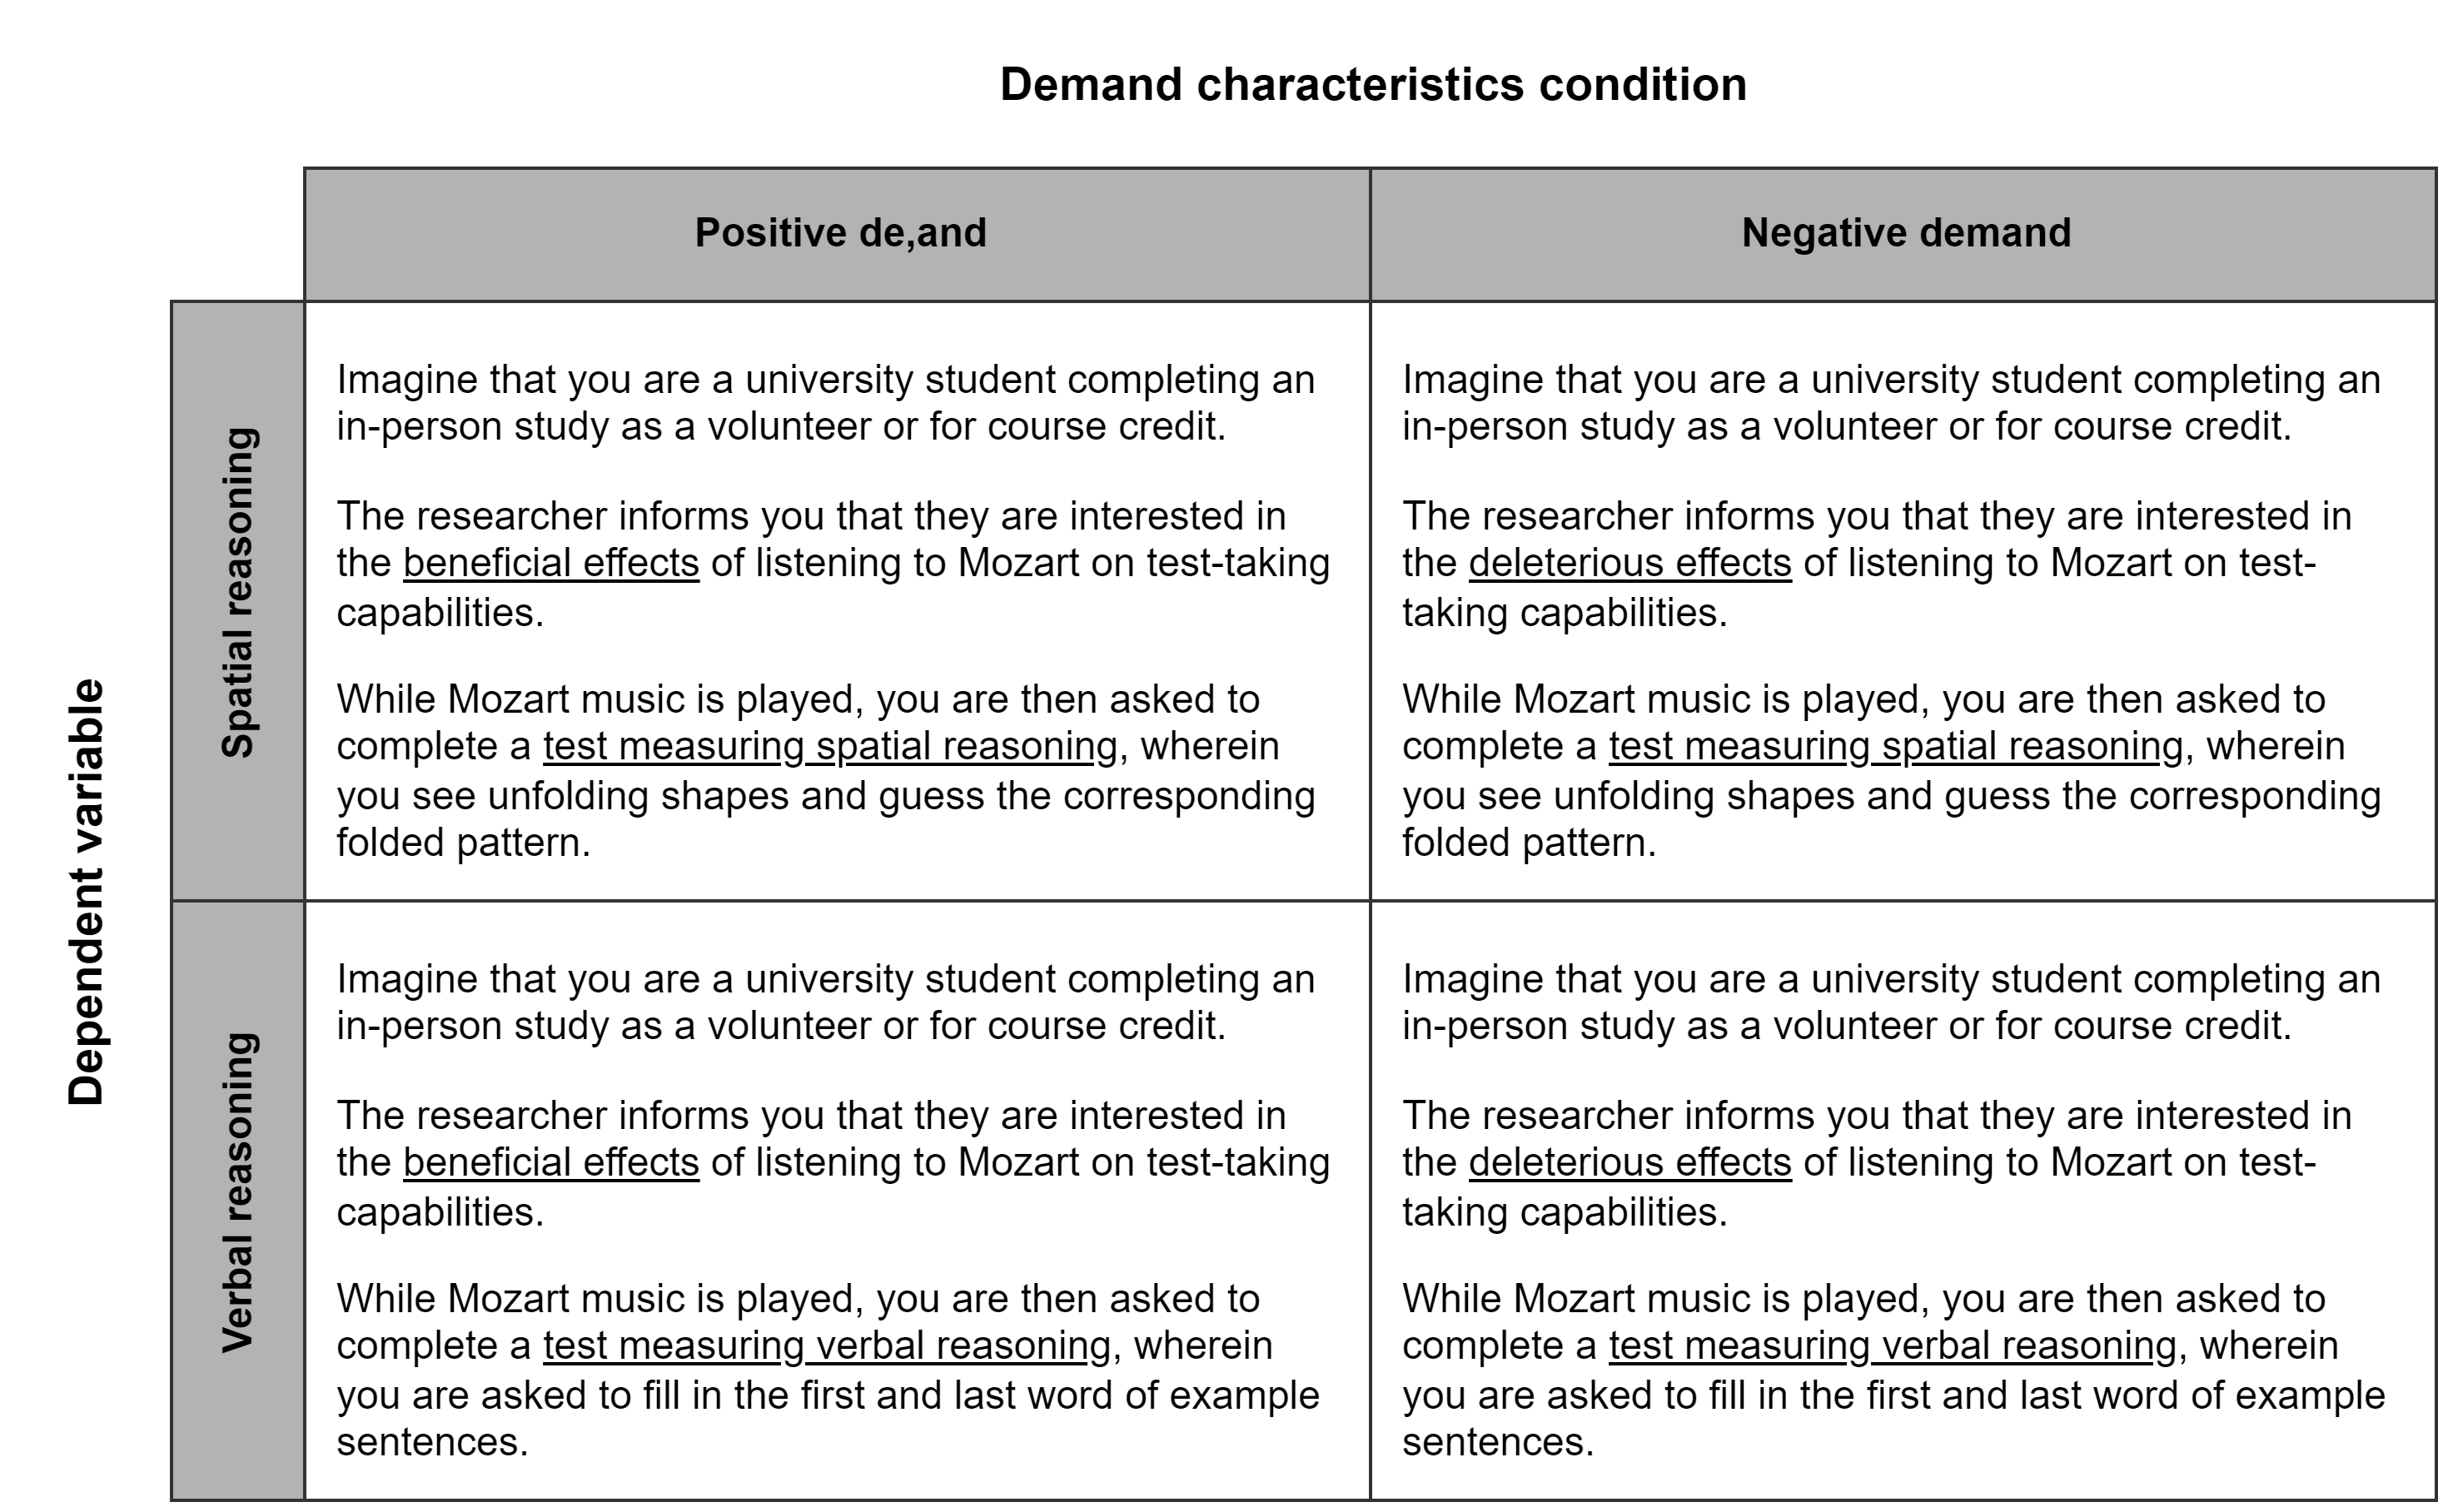
\includegraphics[width=10.01in]{images/metaware_vigs} \caption{Vignettes for Standing et al. (2008), which described the key details for each demand characteristic condition (bolded and underlined) and dependent variable (bolded and italicized) combination.}\label{fig:vig}
\end{figure}

Using a web-based survey, 224 undergraduates from Stanford University reviewed 10 randomly-selected vignettes in exchange for course credit. For each vignette, raters were asked to first identify the researcher's hypothesis. Here, participants chose between four options that described a filler effect (usually involving an irrelevant dependent variable) or a positive, negative, or nil effect of the independent variable on the dependent variable. Afterwards, they rated the extent to which they would hypothetically (1) be motivated to adjust responses based on the hypothesis (-3 = ``extremely motivated to adjust responses to be inconsistent'' to 3 = ``extremely motivated to adjust responses to be consistent''), (2) be able to adjust their responses on the outcome-of-interest (0 = ``extremely incapable'' to 4 = ``extremely capable), and (3) believe the experimenter's hypothesis (-3 =''strong disbelief'' to 3 = ``strong belief''). Raters also indicated whether they believed participants would change their responses to confirm the hypothesis. These questions were presented in random order.

Ratings were removed in instances where the rater did not correctly identify the hypothesis communicated in the vignette. The remaining ratings were averaged across raters to provide mean estimates of motivation, opportunity, and belief.

\begin{figure}
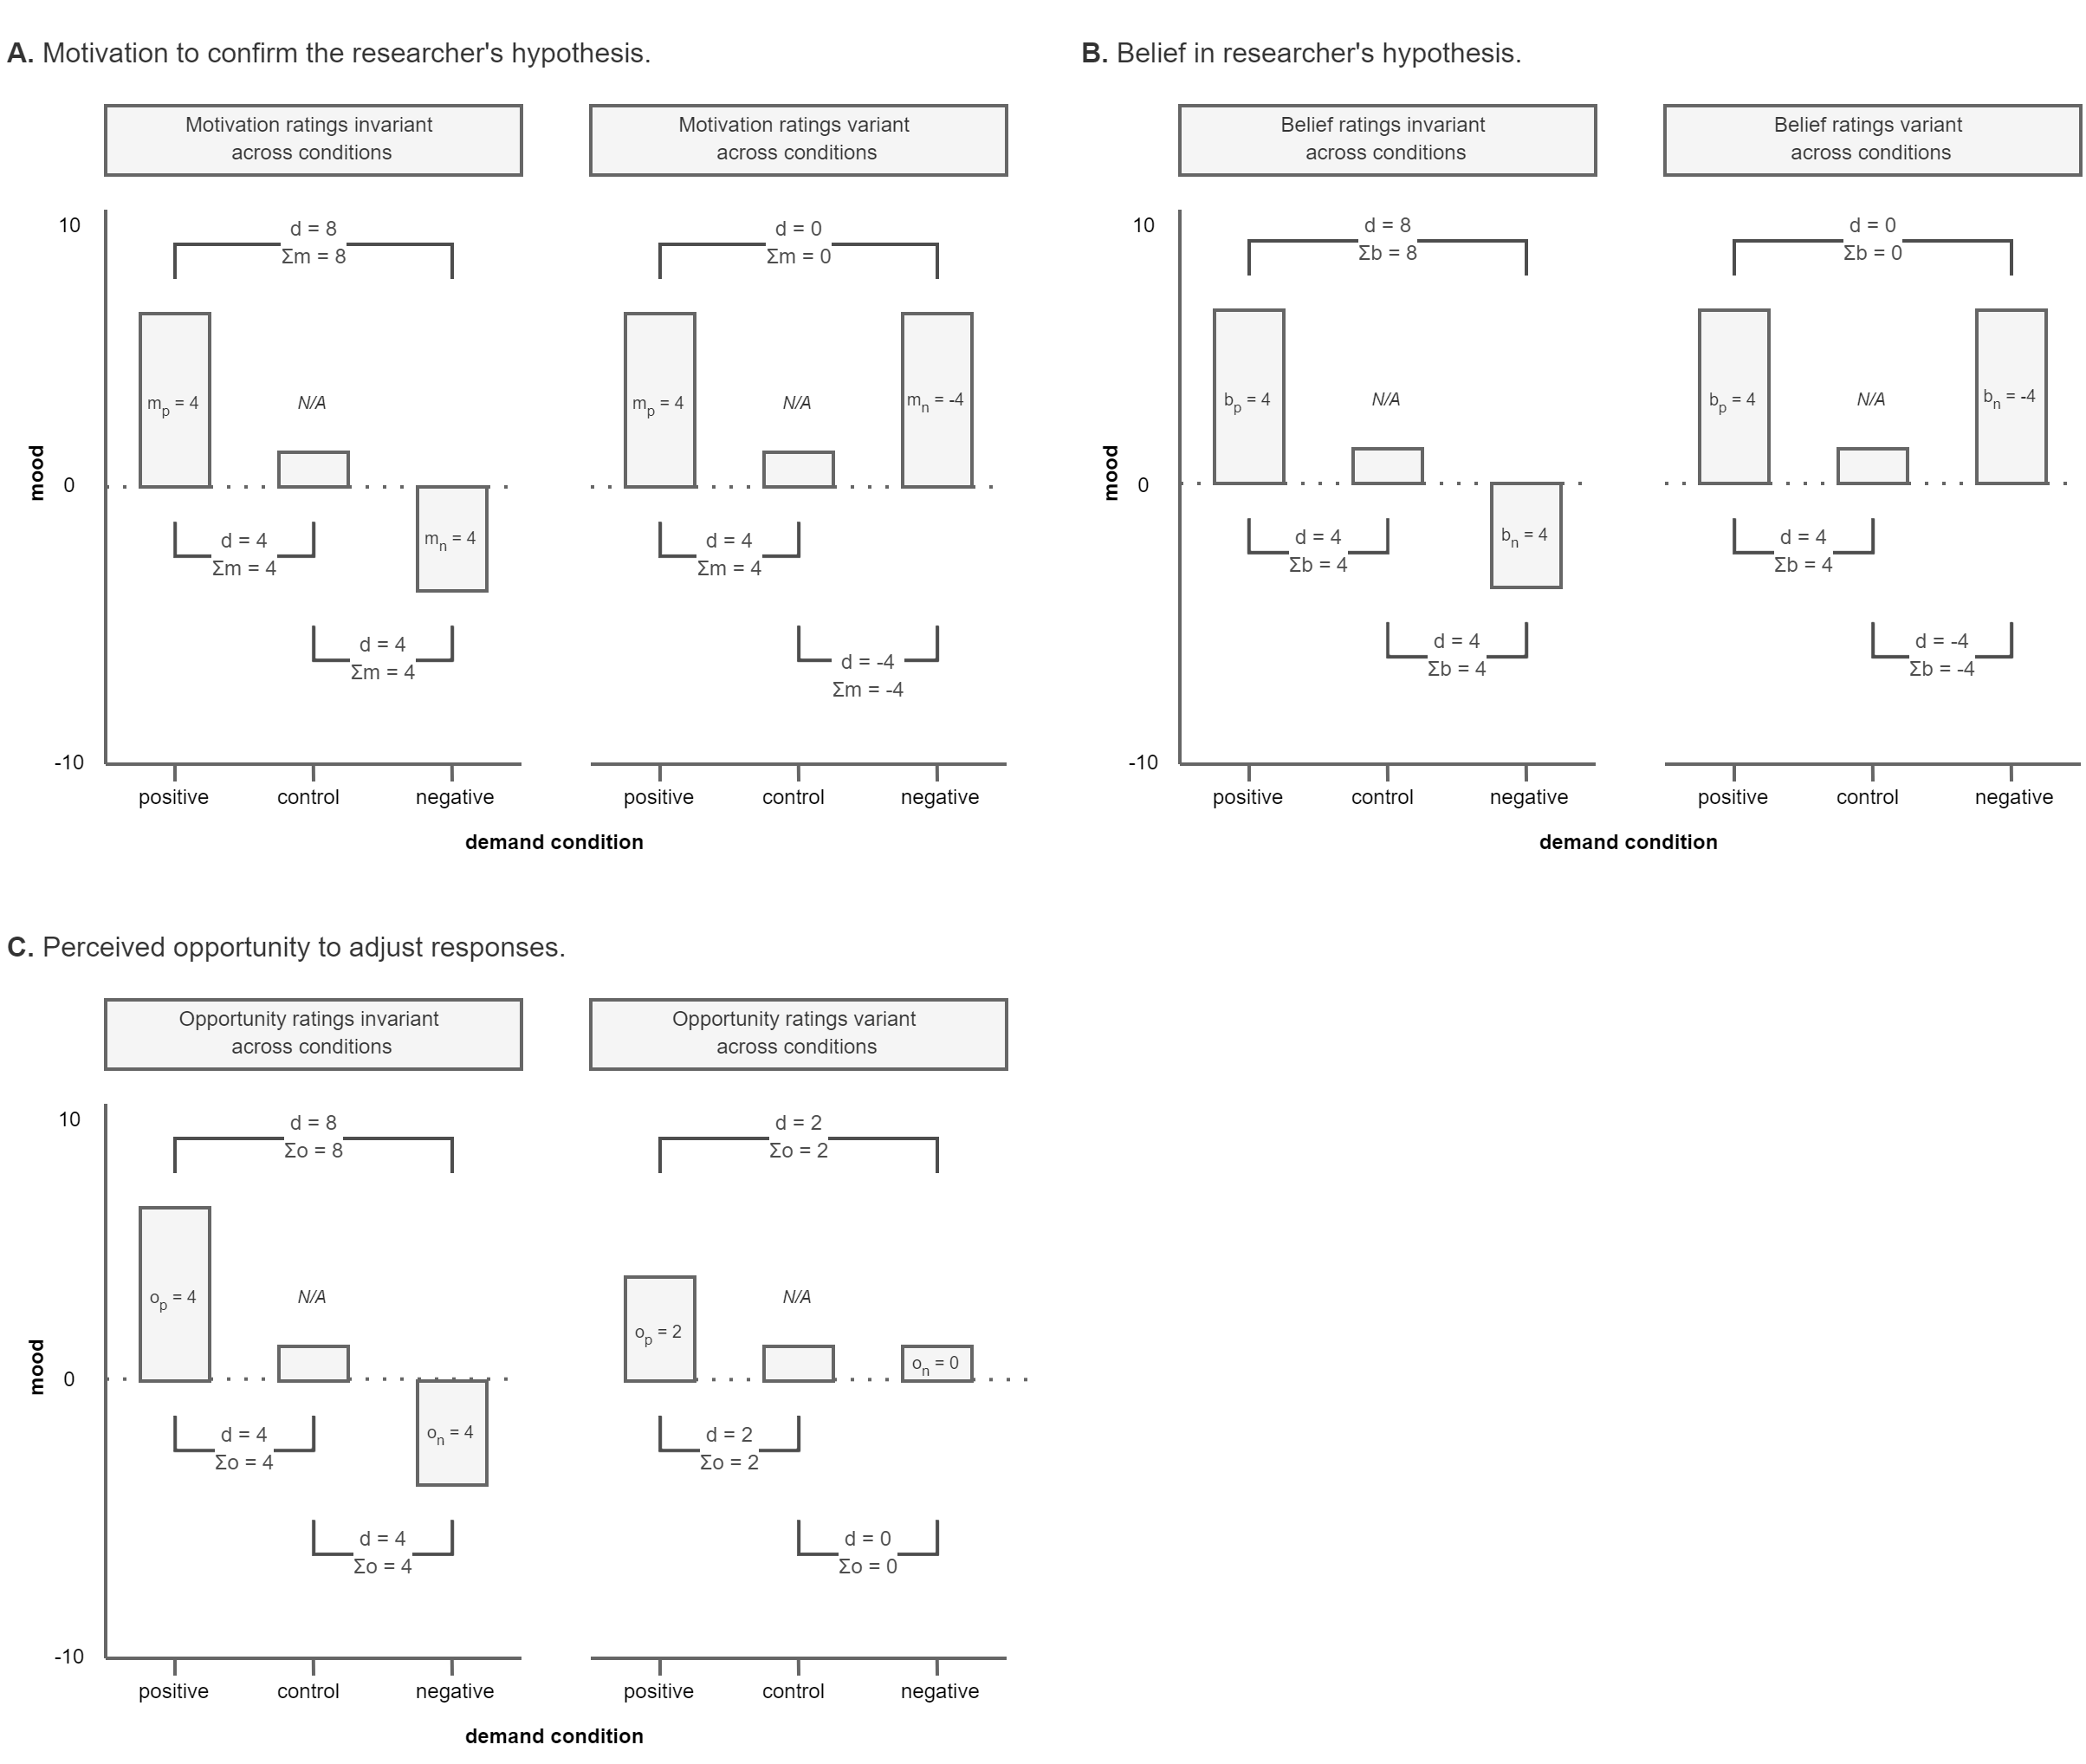
\includegraphics[width=8.03in]{images/metaware_mods} \caption{Hypothetical data from a study where a procedure is either described as mood-boosting (positive demand), described as mood-dampening (negative demand), or not described at all (control). Data provides examples of how the effects of demand characteristics (d) on self-reported mood are moderating by participants' reports of their motivation to confirm the stated hypothesis (m, Panel A), belief in the stated hypothesis (b, Panel B), and opportunity to adjust responses (o, Panel C). In each panel, separate examples are provided for scenarios where motivation is invariant (Column 1) and variant (Column 2) across demand characteristic manipulations}\label{fig:mods}
\end{figure}

\hypertarget{accounting-for-different-demand-comparisons}{%
\subsubsection{Accounting for different demand comparisons}\label{accounting-for-different-demand-comparisons}}

As mentioned before, Cohen's \(d\) represents the standardized difference between \emph{two} groups. Thus, for each effect size estimate, we summed the motivation, opportunity, and belief ratings for the two groups being compared. Doing so allowed us to accommodate the fact that some comparisons involved two demand characteristics conditions. For example, imagine a study where participants are told a procedure will boost mood (positive demand), told a procedure will dampen mood (negative demand), or not told about an expected effect (control). Compared to a control condition, participants who are motivated to confirm the hypothesis are theorized to have upward-biased responses in the positive demand condition and downward-biased responses in the negative demand condition (see Figure \ref{fig:mods}, Panel A, Column 1). When comparing the two demand conditions, the size of the demand effect should be doubled because the motivational forces in the two conditions produce an additive effect. In a different hypothetical context, these motivational forces could cancel each other out. This might happen if participants were (a) motivated to confirm the hypothesis in the positive demand condition, and (b) motivated to \emph{dis}confirm the hypothesis in the negative demand condition (see Figure \ref{fig:mods}, Panel A, Column 2). Summing motivation scores allowed us to accommodate this possibility, and we used the same approach for belief (Figure \ref{fig:mods}, Panel B) and opportunity ratings (Figure \ref{fig:mods}, Panel C).

We did not include nil-hypothesis comparisons in our analyses because our coding strategy could not accommodate the potential moderating role of motivation and belief in these conditions. For example, imagine that a participant is (a) told that an intervention will not impact mood (nil demand), and (b) is extremely motivated to disconfirm the hypothesis. Relative to a control condition, this participant could disconfirm the hypothesis by either increasing \emph{or} decreasing their mood report. Thus, even if motivation does moderate the effects of demand characteristics, we would not expect a systematic pattern to emerge with our coding scheme.

\hypertarget{rater-forecasts-of-demand-effects}{%
\subsubsection{Rater forecasts of demand effects}\label{rater-forecasts-of-demand-effects}}

Even if researchers cannot explain how demand characteristics work, it might be valuable to be able to predict their effects (Yarkoni \& Westfall, 2017). Orne (1969) suggested that one group that may be particularly good at predicting these effects is participants themselves. To examine this, raters also predicted whether other participants would confirm vs.~disconfirm the researcher's hypothesis (-3 = ``extremely likely to adjust responses to be inconsistent'' to 3 = ``extremely likely to adjust responses to be consistent''). We processed these data using the same approach as the motivation, opportunity, and belief scores (e.g., summed ratings when comparing two demand conditions).

\hypertarget{results-1}{%
\subsection{Results}\label{results-1}}

\begin{figure}
\centering
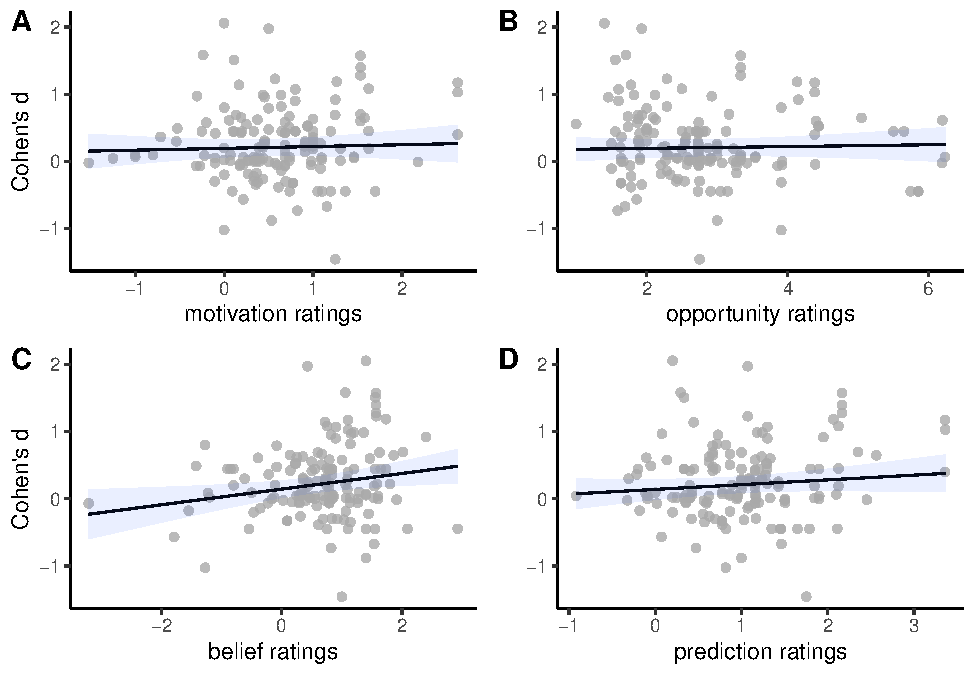
\includegraphics{metaware_manuscript_files/figure-latex/modfig-1.pdf}
\caption{\label{fig:modfig}The effects of demand characteristics on participants' responses were not significantly related to motivation (Panel A), opportunity (Panel B), or prediction (Panel D) ratings. They were, however, significantly related to belief ratings (Panel C).}
\end{figure}

If demand effects are driven by response biases, their effects are expected to be moderated by participants' motivation and opportunity to adjust responses (Figure \ref{fig:framework}). Inconsistent with this view, we did not find that demand effects were moderated by ratings of motivation, \(\beta\) = 0.03, 95\% CI {[}-0.09, 0.14{]}, \(t\)(150) = 0.47, \(p\) = .640) or opportunity to adjust responses, \(\beta\) = 0.01, 95\% CI {[}-0.05, 0.08{]}, \(t\)(150) = 0.40, \(p\) = .689 (Figure \ref{fig:modfig}, Panels A and B).

If demand effects are driven by placebo, their effects should be moderated by participants' belief in the communicated hypothesis. Consistent with this view, demand characteristic effects were positively associated with ratings of belief in the experimenter's hypothesis, \(\beta\) = 0.12, 95\% CI {[}0.02, 0.21{]}, \(t\)(150) = 2.48, \(p\) = .014 (Figure \ref{fig:modfig}, Panel C). Last, we did find that raters' predictions were significantly associated with observed demand effects, \(\beta\) = 0.07, 95\% CI {[}-0.03, 0.17{]}, \(t\)(150) = 1.37, \(p\) = .172 (Figure \ref{fig:modfig}, Panel D).

\hypertarget{residual-variability}{%
\subsubsection{Residual variability}\label{residual-variability}}

To evaluate how much variability in demand effects is currently unaccounted for by our model, we calculated a psuedo-\(R^2\) statistic. We did so by comparing the sum of the variance components (between-study \(\tau^2\) + within-study \(\sigma^2\)) in two 3LMA models: one that contained only an intercept and the other that contained student status, payment status, mode of data collection, type of demand manipulation, belief, motivation, and opportunity as predictors. These results indicated that these moderators accounted for 36.77\% of the observed variability in demand effects.

\hypertarget{discussion-1}{%
\subsection{Discussion}\label{discussion-1}}

Contrary to pre-existing conceptualizations of the impact of demand characteristics Coles, Gaertner, et al. (2022), we did not find evidence of two moderators theorized to underlie a response bias mechanism: motivation and opportunity to adjust responses. We did, however, find evidence that such effects are moderated by a measure of participants' belief in the communicated effect. Given that demand effects appear to depend in part on the extent to which participants' believe the communicated hypothesis, these results provide preliminary evidence of a placebo-based mechanism.

In the current study, we relied on moderator ratings from a new set of participants. This strategy was necessary because researchers have rarely measured these proposed moderators but it has several limitations. First, raters may not have enough information to make an accurate prediction about other participants' motivation, opportunity to adjust responses, and belief in the communicated hypothesis. For the sake of feasibility, we gave participants a short summary of the study, but we don't know how well participants could imagine the reality of being in these studies. Indeed, to gauge the impact of demand characteristics, other researchers have provided participants with extensive information about the study -- even running them through the full procedure (Orne, 1969). Thus, participants might have provided more valid ratings if they had more information about the studies (e.g., video recreations of the procedures).

Second, our specific sample of raters -- or maybe even modern-day participants in general -- may not representative of the people sampled in previous research (Gergen, 1973). In other words, maybe contemporary undergraduates have different study-related motivations, judgments, and beliefs than the participants who completed previous studies on demand characteristics as much as 60 years earlier. To test this idea, we re-ran our motivation, opportunity, and belief moderator analyses focusing only on studies completed in the \emph{past decade}. The idea is that doing so helps minimize differences between the participants who completed the original studies and the raters who completed our rating task. The patterns of results in this sensitivity analysis were largely the same as those from the full dataset.

To address these two limitations via a different strategy, we re-examined the mechanisms underlying demand effects in a small exploratory replication of an experiment in the meta-analysis.

\hypertarget{study-3}{%
\section{Study 3}\label{study-3}}

In addition to the vignette rating task, Study 2 participants also completed an exploratory close replication of Coles, Gaertner, et al. (2022), an experiment on the the effect of facial expressions on feelings of happiness. The order in which participants completed Studies 2 and 3 were randomized.

\hypertarget{methodology-2}{%
\subsection{Methodology}\label{methodology-2}}

We told 222 participants that we hypothesized posed smiles will either increase (positive demand, n = 111) or not impact (nil demand, n = 111) feelings of happiness. Participants then posed happy and neutral expressions across two blocks. For happy poses, participants were instructed to move the corner of their lips toward their ears, elevating their cheeks. For neutral poses, participants were instructed to maintain a blank expression. Participants held each pose for 5 seconds with the assistance of an on-screen timer. After each pose, participants self-reported the extent to which they experienced happiness, satisfaction, and enjoyment (0 = ``not at all'' to 6 = ``maximally''), which were averaged to form a happiness composite score. As filler items, participants also self-reported the extent to which they experienced fear (alarmed, scared, and fear) and anger (irritation, aggravation, and annoyance).

Using a similar procedure as Study 2, participants were excluded if they did not correctly identify the stated hypothesis at the end of the study (final n = 160). Almost all participants correctly inferred that we were interested in links between facial poses and emotional experience. However, particularly in the nil hypothesis condition (76\% of exclusion), they did not correct specify whether we expected a positive or nil effect. Afterwards, participants reported the extent to which they were motivated to confirm the hypothesis, had the opportunity to adjust their responses, and believed in facial feedback effects. These measures were similar to those used in Study 2. Altogether, the study used a 2 (facial pose: happy or neutral) × 2 (block: first or second) × 2 (demand characteristics: positive demand or nil demand) mixed design, with demand characteristics manipulated between subjects.

\hypertarget{results-2}{%
\subsection{Results}\label{results-2}}

Following Coles, Gaertner, et al. (2022), we fit a mixed-effect regression with (a) facial pose, demand characteristics, and block number entered as effect-coded factors and (b) random-intercepts for participants. We used model-derived contrasts to estimate mean differences scores. \emph{F}-values were estimated through ANOVA tables with Type 3 Sums of Squares and Satterthwaite degrees of freedom. Results indicated that participants reported higher levels of happiness after posing happy vs.~neutral expressions, \emph{M\textsubscript{diff}} = 0.71, \emph{F}(1, 469.32) = 162.38, \emph{p} \textless{} .001. Furthermore, this effect was more pronounced in the positive (\emph{M\textsubscript{diff}} = 0.89) vs.~nil (\emph{M\textsubscript{diff}} = 0.52) demand conditions, \emph{F}(1, 469.32) = 11.30, \emph{p =} .001.

Next, we examined the role of motivation, opportunity, and belief. For each of these potential moderators, we fit mixed-effect regressions containing (a) facial pose and block number as effect-coded factors, (b) the moderator entered mean-centered as a continuous variable, (c) a higher-order facial pose by moderator interaction term, and (d) random intercepts for participants. Results indicated that the effect of facial poses on happiness tended to be \emph{slightly} larger among participants who reported being more motivated to confirm the hypothesis, \(\beta\) = 0.04. However, the estimation of this moderating relationship was not significant, \emph{t}(472.40) = 1.86, \emph{p} .063. Furthermore, the estimation of this moderating relationship was less robust when including participants who did not correctly identify the communicated hypothesis, \(\beta\) = 0.03, \emph{t}(585.46) = 1.57, \emph{p =} .117. For ratings of perceived opportunity to adjust responses, we did not find evidence that they moderated the facial pose effect, \(\beta\) = 0.03, \emph{t}(472.15) = 1.36, \emph{p} = .175. However, consistent with previous evidence of placebo effects in facial feedback research (Coles, Gaertner, et al., 2022; Coles, March, et al., 2022), the effect of facial poses tended to be larger among participants who reported believing in the effect, \(\beta\) = 0.05, \emph{t}(472.45) = 2.71, \emph{p} = .007.

The previous analyses provide preliminary evidence that participants' beliefs -- and potentially also their motivation to provide hypothesis consistent responses -- moderate facial feedback effects. They do not, however, test whether these factors drive the effects of \emph{demand characteristics} -- i.e., whether there are three-way interactions between (1) facial poses, (2) demand characteristics, and (3) ratings of motivation, opportunity, and/or belief. For each of these potential moderators, we fit separate mixed-effect regressions containing (a) facial pose and demand characteristics as effect-coded factors, (b) the potential moderator entered mean-centered as a continuous variable, (c) all higher-order interactions, and (d) random intercepts for participants. Results did not indicate that that there was a three-way interaction between facial poses, demand characteristics, and participants' self-reported motivation to provide hypothesis-consistent responses, \(\beta\) = 0.03, \emph{t}(471.24) = 1.20, \emph{p} = .230. We also did not find evidence of a three-way interaction between facial poses, demand characteristics, and participants' self-reported opportunity to adjust responses, \(\beta\) = 0.00, \emph{t}(471.16) = -0.18, \emph{p} = .854. We did, however, find robust evidence of a three-way interaction involving self-reported belief in facial feedback effects. Specifically, the interaction between facial poses and demand characteristics (\(\beta\) = 0.08, \emph{t}(471.22) = 2.79, \emph{p} = .005) tended to be larger among participants with higher belief ratings, \(\beta\) = 0.06, \emph{t}(471.31) = 3.62, \emph{p} \textless{} .001.

To summarize, Study 3 provided little evidence that demand effects are driven by response bias. We found some evidence that facial feedback effects are moderated by self-reported motivation to provide hypothesis-consistent responses -- but this finding was not robust. Furthermore, we consistently failed to find evidence that these effects were moderated by self-reported opportunity to adjust responses. We did, however, find consistent evidence that facial feedback and demand effects are moderated by self-reported belief in the communicated hypothesis.

\hypertarget{general-discussion}{%
\section{General Discussion}\label{general-discussion}}

In our meta-analysis, demand characteristics typically led participants to slightly shift their responses in the direction of the communicated hypothesis. However, publication bias analyses were inconclusive, and the estimated effects were heterogeneous. An estimated 63\% of demand characteristic manipulations produce hypothesis-consistent shifts in participants' responses (\(d\) \textgreater{} 0.10), 19\% produce hypothesis-\emph{in}consistent shifts in participants' responses (\(d\) \textless{} -0.10), and 18\% produce negligible shifts in either direction (-0.10 \textless{} \(d\) \textgreater{} 0.10). Most worrisome, the current estimated distribution of demand effects suggests that they can range from approximately \(d\) = -1.48 to \(d\) = 2.10. This distribution is remarkably similar to the distribution of theory-relevant effects in experimental psychology (Lovakov \& Agadullina, 2021). Thus, in order to distinguish theory-relevant effects from artifactual demand effects, it is essential that experimental psychologists better understand demand.

Participants themselves appeared to have little ability to predict the impact of demand characteristics in the studies they reviewed, although it is possible that their performance would improve if they were provided with more information, given better measures, and/or better incentivized to provide accurate predictions. Fortunately, our meta-analysis allows us to make some predictions. Moderator analyses provided preliminary evidence that some methodological decisions -- such as sampling students, running studies in-person, and not offering payment -- are associated with increases in hypothesis-consistent responding. We also found that demand characteristics tended to be more impactful when a nil (as opposed to negative or positive) hypothesis was communicated. Nonetheless, most of the variability we observed in the meta-analysis was not predictable.

On the other hand, we found robust evidence that demand effects are at least partly driven by participants' beliefs about the study they are participating in. This finding challenges historical distinctions made between placebo effects and demand characteristics -- the later which have been conventionally conceptualized as a relatively deliberate response bias driven by participants' motivation and ability to adjust their responses (Cook et al., 1970; Orne, 1962; Riecken, 1962; Rosenberg, 1969; Rosnow \& Rosenthal, 1997; Sigall et al., 1970). Contrary to these conventional conceptualizations, we did not find much evidence that demand characteristics are driven by response bias. In the Study 2 meta-analysis, we did not find that external ratings of two factors theorized to underlie response biases -- motivation and opportunity to adjust responses -- moderated demand effects. We found some evidence in Study 3 that motivation (but not opportunity) ratings moderated demand effects, but the evidence was weak.

On the basis of this evidence, we suggest that it is no longer tenable to keep demand characteristics conceptually divorced from related work on placebo effects. Consistent with recently proposed extensions of demand characteristic frameworks, our meta-analysis and replication study consistently indicated that participants' beliefs partially drive demand effects (Coles, Gaertner, et al., 2022; Corneille \& Lush, 2022). This may occur because demand characteristics activate pre-existing beliefs about a phenomenon being investigated. It is also possible that demand characteristics cause participants to update or form new beliefs. If true, research on how beliefs are formed, updated, and impact participant responses may help explain the unreliable effects of demand characteristic manipulations. For example, if beliefs are governed by Bayesian principles (for a review, see Kube \& Rozenkrantz, 2021), demand characteristics should exert larger effects in contexts where participants have relatively uncertain pre-existing beliefs.

Placebo effects can certainly be reduced -- but it is not clear if they can be fully avoided. Existing demand characteristic frameworks suggest that placebo effects can be diminished by reducing receptivity (e.g., by using deception). However, it is important to note that participants' possess a rich array of pre-existing beliefs \emph{before} they enter our studies (Dweck, 2012). For example, Coles, Gaertner, et al. (2022) estimated that 44\% of sampled undergraduates and 34\% of sampled online workers believed -- before entering the study -- that facial poses impact emotion. Even with deception about the purpose of the study, these pre-existing beliefs appear to shape the extent to which participants exhibit facial feedback effects. In other words, deception about the purpose the study does not guarantee an unbiased estimate of a mechanism-of-interest. In the real world, the mechanisms that psychologists theorize about may be naturalistically confounded with participants' beliefs.

We end on a note of concern. We estimated that experimentally manipulated demand characteristics have a similar distribution of effects as the theory-relevant phenomena that psychologists study (Lovakov \& Agadullina, 2021). These demand effects appear to be most robustly driven by participant beliefs (i.e., placebo effects). Even when specific demand characteristics are eliminated, participants possess beliefs about the phenomena we study -- and these beliefs may be naturalistically confounded with the theory-relevant mechanisms we wish to study. Thus, if (a) demand characteristics are present or (b) participants' are likely to posess pre-existing beliefs about the phenomenon being studied, researchers should be wary of concluding that an observed effect is not compromised by methodological artifact. To make conclusions about theory-relevant mechanisms, demand characteristics must be eliminated, beliefs must be controlled, and direct evidence for mechanisms must be provided.

\hypertarget{references}{%
\section{References}\label{references}}

\hypertarget{refs}{}
\begin{CSLReferences}{1}{0}
\leavevmode\vadjust pre{\hypertarget{ref-allen2012demand}{}}%
Allen, A. P., \& Smith, A. P. (2012). Demand characteristics, pre-test attitudes and time-on-task trends in the effects of chewing gum on attention and reported mood in healthy volunteers. \emph{Appetite}, \emph{59}(2), 349--356.

\leavevmode\vadjust pre{\hypertarget{ref-berkowitz1971weapons}{}}%
Berkowitz, L. (1971). The" weapons effect," demand characteristics, and the myth of the compliant subject. \emph{Journal of Personality and Social Psychology}, \emph{20}, 332--338.

\leavevmode\vadjust pre{\hypertarget{ref-borenstein2009effect}{}}%
Borenstein, M. (2009). Effect sizes for continuous data. In H. Cooper, L. V. Hedges, \& J. C. Valentine (Eds.), \emph{The handbook of synthesis and meta-analysis} (pp. 221--235). New York, NY: Russell Sage Foundation.

\leavevmode\vadjust pre{\hypertarget{ref-borenstein2011introduction}{}}%
Borenstein, M., Hedges, L. V., Higgins, J. P., \& Rothstein, H. R. (2011). \emph{Introduction to meta-analysis}. John Wiley \& Sons.

\leavevmode\vadjust pre{\hypertarget{ref-cohen1988statistical}{}}%
Cohen, J. (2013). \emph{Statistical power analysis for the behavioral sciences} (Vol. 2). New York, NY: Lawrence Erlbaum Associates.

\leavevmode\vadjust pre{\hypertarget{ref-coles2022fact}{}}%
Coles, N. A., Gaertner, L., Frohlich, B., Larsen, J. T., \& Basnight-Brown, D. M. (2022). Fact or artifact? Demand characteristics and participants' beliefs can moderate, but do not fully account for, the effects of facial feedback on emotional experience. \emph{Journal of Personality and Social Psychology}.

\leavevmode\vadjust pre{\hypertarget{ref-coles2019meta}{}}%
Coles, N. A., Larsen, J. T., \& Lench, H. C. (2019). A meta-analysis of the facial feedback literature: Effects of facial feedback on emotional experience are small and variable. \emph{Psychological Bulletin}, \emph{145}(6), 610--651.

\leavevmode\vadjust pre{\hypertarget{ref-coles2022multi}{}}%
Coles, N. A., March, D. S., Marmolejo-Ramos, F., Larsen, J. T., Arinze, N. C., Ndukaihe, I. L., et al.others. (2022). A multi-lab test of the facial feedback hypothesis by the many smiles collaboration. \emph{Nature Human Behaviour}, 1--12.

\leavevmode\vadjust pre{\hypertarget{ref-cook1970demand}{}}%
Cook, T. D., Bean, J. R., Calder, B. J., Frey, R., Krovetz, M. L., \& Reisman, S. R. (1970). Demand characteristics and three conceptions of the frequently deceived subject. \emph{Journal of Personality and Social Psychology}, \emph{14}(3), 185--194.

\leavevmode\vadjust pre{\hypertarget{ref-corneille2022sixty}{}}%
Corneille, O., \& Lush, P. (2022). Sixty years after orne's american psychologist article: A conceptual framework for subjective experiences elicited by demand characteristics. \emph{Personality and Social Psychology Review}, 81--101.

\leavevmode\vadjust pre{\hypertarget{ref-drevon2017intercoder}{}}%
Drevon, D., Fursa, S. R., \& Malcolm, A. L. (2017). Intercoder reliability and validity of WebPlotDigitizer in extracting graphed data. \emph{Behavior Modification}, \emph{41}(2), 323--339.

\leavevmode\vadjust pre{\hypertarget{ref-dweck2012implicit}{}}%
Dweck, C. S. (2012). Implicit theories. In P. A. M. V. Lange, A. W. Kruglanski, \& T. Higgins (Eds.), \emph{Handbook of theories of social psychology} (Vol. 2, pp. 43--61). London: SAGE Publications Ltd.

\leavevmode\vadjust pre{\hypertarget{ref-fillenbaun1970more}{}}%
Fillenbaun, S., \& Frey, R. (1970). More on the" faithful" behavior of suspicious subjects. \emph{Journal of Personality}, \emph{38}(1), 43--51.

\leavevmode\vadjust pre{\hypertarget{ref-franco2014publication}{}}%
Franco, A., Malhotra, N., \& Simonovits, G. (2014). Publication bias in the social sciences: Unlocking the file drawer. \emph{Science}, \emph{345}(6203), 1502--1505.

\leavevmode\vadjust pre{\hypertarget{ref-gergen1973social}{}}%
Gergen, K. J. (1973). Social psychology as history. \emph{Journal of Personality and Social Psychology}, \emph{26}(2), 309.

\leavevmode\vadjust pre{\hypertarget{ref-greenwald1998measuring}{}}%
Greenwald, A. G., McGhee, D. E., \& Schwartz, J. L. (1998). Measuring individual differences in implicit cognition: The implicit association test. \emph{Journal of Personality and Social Psychology}, \emph{74}(6), 1464.

\leavevmode\vadjust pre{\hypertarget{ref-hayes1967two}{}}%
Hayes, C., \& King, W. (1967). Two types of phenomenal instructions for size and distance judgments of objects presented on a two-dimensional plane. \emph{Perception \& Psychophysics}, \emph{2}(11), 556--558.

\leavevmode\vadjust pre{\hypertarget{ref-kenealy1988validation}{}}%
Kenealy, P. (1988). Validation of a music mood induction procedure: Some preliminary findings. \emph{Cognition \& Emotion}, \emph{2}(1), 41--48.

\leavevmode\vadjust pre{\hypertarget{ref-kruglanski1975human}{}}%
Kruglanski, A. W. (1975). The human subject in the psychology experiment: Fact and artifact. \emph{Advances in Experimental Social Psychology}, \emph{8}, 101--147.

\leavevmode\vadjust pre{\hypertarget{ref-kube2021beliefs}{}}%
Kube, T., \& Rozenkrantz, L. (2021). When beliefs face reality: An integrative review of belief updating in mental health and illness. \emph{Perspectives on Psychological Science}, \emph{16}(2), 247--274.

\leavevmode\vadjust pre{\hypertarget{ref-lovakov2021empirically}{}}%
Lovakov, A., \& Agadullina, E. R. (2021). Empirically derived guidelines for effect size interpretation in social psychology. \emph{European Journal of Social Psychology}, \emph{51}(3), 485--504.

\leavevmode\vadjust pre{\hypertarget{ref-masling1966role}{}}%
Masling, J. (1966). Role-related behavior of the subject and psychologist and its effects upon psychological data. \emph{Nebraska Symposium on Motivation}, \emph{14}, 67--103.

\leavevmode\vadjust pre{\hypertarget{ref-milgram1972interpreting}{}}%
Milgram, S. (1972). Interpreting obedience: Error and evidence. A reply to orne and holland. In A. G. Miller (Ed.), \emph{The social psychology of psychological research} (pp. 138--154). New York, NY: Free Press.

\leavevmode\vadjust pre{\hypertarget{ref-mummolo2019demand}{}}%
Mummolo, J., \& Peterson, E. (2019). Demand effects in survey experiments: An empirical assessment. \emph{American Political Science Review}, \emph{113}(2), 517--529.

\leavevmode\vadjust pre{\hypertarget{ref-orne1959nature}{}}%
Orne, M. T. (1959). The nature of hypnosis: Artifact and essence. \emph{The Journal of Abnormal and Social Psychology}, \emph{58}(3), 277--299.

\leavevmode\vadjust pre{\hypertarget{ref-orne1962social}{}}%
Orne, M. T. (1962). On the social psychology of the psychological experiment: With particular reference to demand characteristics and their implications. \emph{American Psychologist}, \emph{17}(11), 776--783.

\leavevmode\vadjust pre{\hypertarget{ref-orne1969demand}{}}%
Orne, M. T. (1969). Demand characteristics and the concept of quasi-controls. In R. Rosenthal \& R. L. Rosnow (Eds.), \emph{Artifacts in behavioral research} (pp. 143--179). New York, NY: Academic Press.

\leavevmode\vadjust pre{\hypertarget{ref-riecken1962program}{}}%
Riecken, H. W. (1962). A program for research on experiments in social psychology. In N. W. Washburne (Ed.), \emph{Decisions, values and groups} (Vol. 2, pp. 25--41). New York, NY: Pergamon Press.

\leavevmode\vadjust pre{\hypertarget{ref-rodgers2021evaluating}{}}%
Rodgers, M. A., \& Pustejovsky, J. E. (2021). Evaluating meta-analytic methods to detect selective reporting in the presence of dependent effect sizes. \emph{Psychological Methods}, \emph{26}(2), 141.

\leavevmode\vadjust pre{\hypertarget{ref-rosenberg1969conditions}{}}%
Rosenberg, M. J. (1969). The conditions and consequences of evaluation apprehension. In R. Rosenthal \& R. L. Rosnow (Eds.), \emph{Artifacts in behavioral research} (pp. 280--350). New York, NY: Academic Press.

\leavevmode\vadjust pre{\hypertarget{ref-rosnow1973mediation}{}}%
Rosnow, R. L., \& Aiken, L. S. (1973). Mediation of artifacts in behavioral research. \emph{Journal of Experimental Social Psychology}, \emph{9}(3), 181--201.

\leavevmode\vadjust pre{\hypertarget{ref-rosnow1997people}{}}%
Rosnow, R. L., \& Rosenthal, R. (1997). \emph{People studying people: Artifacts and ethics in behavioral research}. New York, NY: Freeman.

\leavevmode\vadjust pre{\hypertarget{ref-schardt2007utilization}{}}%
Schardt, C., Adams, M. B., Owens, T., Keitz, S., \& Fontelo, P. (2007). Utilization of the PICO framework to improve searching PubMed for clinical questions. \emph{BMC Medical Informatics and Decision Making}, \emph{7}(1), 1--6.

\leavevmode\vadjust pre{\hypertarget{ref-sharpe2016frightened}{}}%
Sharpe, D., \& Whelton, W. J. (2016). Frightened by an old scarecrow: The remarkable resilience of demand characteristics. \emph{Review of General Psychology}, \emph{20}(4), 349--368.

\leavevmode\vadjust pre{\hypertarget{ref-sigall1970cooperative}{}}%
Sigall, H., Aronson, E., \& Van Hoose, T. (1970). The cooperative subject: Myth or reality? \emph{Journal of Experimental Social Psychology}, \emph{6}(1), 1--10.

\leavevmode\vadjust pre{\hypertarget{ref-standing2008demonstration}{}}%
Standing, L. G., Verpaelst, C. C., \& Ulmer, B. K. (2008). A demonstration of nonlinear demand characteristics in the'mozart effect'experimental paradigm. \emph{North American Journal of Psychology}, \emph{10}(3), 553--566.

\leavevmode\vadjust pre{\hypertarget{ref-stanley2014meta}{}}%
Stanley, T. D., \& Doucouliagos, H. (2014). Meta-regression approximations to reduce publication selection bias. \emph{Research Synthesis Methods}, \emph{5}(1), 60--78.

\leavevmode\vadjust pre{\hypertarget{ref-strohmetz2008research}{}}%
Strohmetz, D. B. (2008). Research artifacts and the social psychology of psychological experiments. \emph{Social and Personality Psychology Compass}, \emph{2}(2), 861--877.

\leavevmode\vadjust pre{\hypertarget{ref-vevea1995general}{}}%
Vevea, J. L., \& Hedges, L. V. (1995). A general linear model for estimating effect size in the presence of publication bias. \emph{Psychometrika}, \emph{60}(3), 419--435.

\leavevmode\vadjust pre{\hypertarget{ref-yarkoni2017choosing}{}}%
Yarkoni, T., \& Westfall, J. (2017). Choosing prediction over explanation in psychology: Lessons from machine learning. \emph{Perspectives on Psychological Science}, \emph{12}(6), 1100--1122.

\leavevmode\vadjust pre{\hypertarget{ref-zion2018mindsets}{}}%
Zion, S. R., \& Crum, A. J. (2018). Mindsets matter: A new framework for harnessing the placebo effect in modern medicine. \emph{International Review of Neurobiology}, \emph{138}, 137--160.

\end{CSLReferences}


\end{document}
